\section{Further experimental details}
\label{app:further-exp-details}

In this section, we provide additional details and results for our experiments. First we provide more details about the vector field reconstruction task. Then, we provide the summary table for the forecasting and interpolation task for all experiments using EMD. After that, for each experiment introduced in the main text, we describe: (1) the experimental setup, (2) the choice of model family used with our method, (3) forecasting results, (4) vector field reconstruction results, and (5) interpolation results. Our experiments are carried out using four cores of Intel Xeon Gold 6248 CPU and one Nvidia Volta V100 GPU with 32 GB RAM.


\subsection{Vector Field Reconstruction}
\label{app:vector-field-reconstruction}
In cases where the true underlying drift function is known (e.g., synthetic experiments), we also evaluate how accurately methods reconstruct the vector field driving the system dynamics. We use the same baselines as in the forecasting task, since this task also requires recovering a coherent forward-time dynamic, rather than just interpolating between marginals. We measure reconstruction accuracy visually and by computing mean squared error (MSE) between the learned drift and ground truth drift on a dense grid covering the observed data range. Overall, our method provides better or matching vector field reconstruction performance relative to competitors. Detailed results for vector field reconstruction are presented in \cref{app:lv-vector} (for Lotka-Volterra), \cref{app:repr-vector-parametric} (for repressilator with parametric model family), \cref{app:repr-vector-semiparametric} (for repressilator with semiparametric model family), and \cref{app:gom-vector} (for Gulf of Mexico). 

\subsection{How we use $R^2$ in our experiments}
\label{app:use-r2-experiments}
In this section, we briefly describe how the proposed $R^2$ metric is used in our experiments. The \(R^2\) metric defined in \cref{eq:R2_metric} naturally provides a standardized and interpretable criterion to compare candidate SDE models, guiding model selection and diagnosing fit quality. Values of \(R^2\) close to 1 indicate a high-quality fit, while values near or below 0 signal poor model performance relative to the simple barycenter model. Finally, note that \(R^2\) is always upper bounded by 1 due to the non-negativity of the MMD, and it may become negative if the candidate model performs worse than the barycenter, analogous to regression models without an intercept. In our experiments, we apply it in two main ways. First, for early stopping: we select the number of training epochs such that $R^2$ increases by less than 0.01 over the last 20 epochs. Second, as a model selection criterion when choosing among neural network architectures. In particular, for real-data experiments using multilayer perceptrons, we perform a small grid search over the number of layers and hidden units, selecting the model with the highest $R^2$. Specific details for each experiment are provided in the “Model family choice” subsections in \cref{app:further-exp-details}.

\subsection{EMD table with summary results across all methods and experiments}
\label{app:emd-big-table}
In this section, we provide the summary table (\cref{tab:emd_combined}) for comparing forecasting and interpolation performance in terms of EMD over all the experiments of interest. For the interpolation results, we report the mean and standard deviation for each method, aggregated over different random seeds and interpolation held-out time points. Detailed per-time-point results are provided for each experiment in the corresponding “Interpolation results” subsubsection later in \cref{app:further-exp-details}. 

\begin{table}[!ht]
\caption{EMD for forecast and interpolation tasks.  Bold green = best method; plain green = method whose mean lies within one standard deviation of the best method. }
\centering
\makebox[0pt][c]{
\small
\begin{tabular}{lcccccc}
\toprule
      & \multicolumn{3}{c}{\textbf{Forecast}} & \multicolumn{3}{c}{\textbf{Interpolation}} \\
\cmidrule(lr){2-4}\cmidrule(lr){5-7}
\textbf{Task}
      & \textbf{Ours} & \texttt{SBIRR-ref} & \texttt{SB-forward}
      & \textbf{Ours} & \texttt{SBIRR} & \texttt{DMSB} \\ \midrule
LV
      & \best{\ms{0.21}{0.04}} & \ms{0.79}{0.05} & \ms{1.82}{0.9}
      & \best{\ms{0.06}{0.03}} & \ms{0.10}{0.08} & \ms{0.82}{0.6} \\ \midrule
ReprParam
      & \best{\ms{0.19}{0.08}} & \ms{1.55}{0.8} & \ms{1.39}{0.6}
      & \best{\ms{0.10}{0.04}} & \ms{0.17}{0.06} & \ms{1.89}{0.9} \\
ReprSemiparam
      & \best{\ms{0.35}{0.09}} & \ms{1.18}{0.4} & \ms{1.16}{0.3}
      & \best{\ms{0.21}{0.11}} & \ms{0.39}{0.1} & \ms{1.89}{0.9} \\
ReprProtein
      & \best{\ms{0.26}{0.04}} & \ms{6.36}{0.5} & \ms{7.24}{0.5}
      & \best{\ms{0.08}{0.03}} & \ms{0.59}{0.8} & \ms{1.48}{1.0} \\ \midrule
GoM
      & \best{\ms{0.71}{0.01}} & \ms{0.89}{0.03} & \ms{0.94}{0.08}
      & \ms{0.10}{0.04} & \best{\ms{0.04}{0.01}} & \ms{0.08}{0.04} \\ \midrule
PBMC
      & -- & -- & --  & -- & -- & -- \\
\bottomrule
\end{tabular}}
\label{tab:emd_combined}
\end{table}


\subsection{Full results for interpolation task}
\label{app:complete-summary-interpolation}
In this section, we provide summary tables for all methods for the interpolation task. In \cref{tab:interp-summary-complete-mmd} we provide the summary table for MMD. In \cref{tab:interp-summary-complete-emd} we provide the summary table for EMD. As in \cref{app:emd-big-table}, we report the mean and standard deviation for each method, aggregated over different random seeds and interpolation held-out time points. We find that in almost all experiments, SnapMMD provides better or matching interpolation performance relative to competitors.

\begin{table}[!hb]
\caption{Global summary of MMD across all seeds and validation points}
\centering
\makebox[0pt][c]{
\small
\begin{tabular}{lrrrrrr}
\toprule
Task & Ours & \texttt{SBIRR} & \texttt{DMSB} & \texttt{OT-CFM} & \texttt{SB-CFM} & \texttt{SF2M} \\\midrule
LV & \cellcolor{green!25}\bm{$0.013\pm{\scriptsize 0.011}$} & $0.048\pm{\scriptsize 0.082}$ & $3.316\pm{\scriptsize 2.175}$ & $2.830\pm{\scriptsize 2.929}$ & $2.099\pm{\scriptsize 2.245}$ & $2.055\pm{\scriptsize 1.915}$ \\
ReprParam & \cellcolor{green!25}\bm{$0.040\pm{\scriptsize 0.034}$} & $0.156\pm{\scriptsize 0.102}$ & $7.269\pm{\scriptsize 2.001}$ & $4.639\pm{\scriptsize 2.123}$ & $3.500\pm{\scriptsize 1.878}$ & $3.327\pm{\scriptsize 1.157}$ \\
ReprSemiparam & \cellcolor{green!25}\bm{$0.379\pm{\scriptsize 0.381}$} & $1.105\pm{\scriptsize 0.815}$ & $7.269\pm{\scriptsize 2.001}$ & $4.639\pm{\scriptsize 2.123}$ & $3.500\pm{\scriptsize 1.878}$ & $3.327\pm{\scriptsize 1.157}$ \\
ReprProtein & \cellcolor{green!25}\bm{$0.011\pm{\scriptsize 0.006}$} & $1.480\pm{\scriptsize 2.953}$ & $5.147\pm{\scriptsize 2.630}$ & $4.092\pm{\scriptsize 3.086}$ & $2.878\pm{\scriptsize 2.643}$ & $3.091\pm{\scriptsize 2.582}$ \\
Gulf of Mexico & $0.073\pm{\scriptsize 0.054}$ & \cellcolor{green!25}\bm{$0.008\pm{\scriptsize 0.009}$} & $0.053\pm{\scriptsize 0.064}$ & $0.651\pm{\scriptsize 0.443}$ & $0.693\pm{\scriptsize 0.564}$ & $0.624\pm{\scriptsize 0.406}$ \\
PBMC & \cellcolor{green!25}\bm{$0.114\pm{\scriptsize 0.052}$} & \cellcolor{green!25}$0.114\pm{\scriptsize 0.122}$ & $0.968\pm{\scriptsize 0.095}$ & $0.440\pm{\scriptsize 0.195}$ & $0.488\pm{\scriptsize 0.198}$ & $0.343\pm{\scriptsize 0.094}$ \\
\bottomrule
\end{tabular}}
\label{tab:interp-summary-complete-mmd}
\end{table}



\begin{table}[!hb]
\caption{Global summary of EMD across all seeds and validation points. For the repressilator with incomplete state measurements, for some random seeds the trajectories generated by SB-CFM and SF2M diverged significantly, leading to extremely large average EMD values ($1138.222 \pm 8653.586$ for SB-CFM and $1954.050 \pm 14737.310$ for SF2M). To maintain visualization clarity, we omit these entries from the summary table.}
\centering
\makebox[0pt][c]{
\small
\begin{tabular}{lrrrrrr}
\toprule
Task & Ours & \texttt{SBIRR} & \texttt{DMSB} & \texttt{OT-CFM} & \texttt{SB-CFM} & \texttt{SF2M} \\\midrule
LV & \cellcolor{green!25}\bm{$0.064\pm{ 0.031}$} & $0.096\pm{ 0.075}$ & $0.819\pm{ 0.559}$ & $0.742\pm{ 0.698}$ & $0.669\pm{ 0.674}$ & $0.770\pm{ 0.706}$ \\
ReprParam & \cellcolor{green!25}\bm{$0.096\pm{ 0.041}$} & $0.168\pm{ 0.057}$ & $1.887\pm{ 0.865}$ & $1.367\pm{ 0.793}$ & $1.412\pm{ 1.377}$ & $23.201\pm{ 122.101}$ \\
ReprProtein & \cellcolor{green!25}\bm{$0.080\pm{ 0.032}$} & $0.591\pm{ 0.783}$ & $1.480\pm{ 1.011}$ & $1.328\pm{ 1.026}$ & -- & -- \\
ReprSemiparam & \cellcolor{green!25}\bm{$0.210\pm{ 0.106}$} & $0.394\pm{ 0.136}$ & $1.887\pm{ 0.865}$ & $1.367\pm{ 0.793}$ & $1.412\pm{ 1.377}$ & $23.201\pm{ 122.101}$ \\
Gulf of Mexico & $0.103\pm{ 0.040}$ & \cellcolor{green!25}\bm{$0.043\pm{ 0.012}$} & $0.078\pm{ 0.037}$ & $0.252\pm{ 0.109}$ & $0.265\pm{ 0.136}$ & $0.249\pm{ 0.102}$ \\
PBMC & -- & -- & -- & -- & -- & -- \\
\bottomrule
\end{tabular}}
\label{tab:interp-summary-complete-emd}
\end{table}



\clearpage

\subsection{Lotka-Volterra}
\label{app:lv-app}
\subsubsection{Experiment setup}
In this experiment, we study the stochastic Lotka-Volterra model, which describes predator-prey interactions over time. The population dynamics are governed by the following system of SDEs:
\begin{align}
\begin{split}
\label{eq:lv-family}
    dX &= \alpha X - \beta XY + \sigma X dW_x, \\
    dY &= \gamma XY - \delta Y + \sigma Y dW_y,
\end{split}
\end{align}
where $[dW_x, dW_y]$ denotes a two-dimensional Brownian motion. The true parameter values are set to $\alpha = 1.0$, $\beta = 0.4$, $\gamma = 0.4$, $\delta = 0.1$, and $\sigma = 0.02$. Initial population sizes are sampled from uniform distributions: $X_0 \sim U(5, 5.1)$ and $Y_0 \sim U(4, 4.1)$. We simulate the system over 19 discrete time points using the Euler–Maruyama method (via the \texttt{torchsde} Python package), with a time step of 0.5 and 200 samples per time point. We use the 10 odd-numbered time steps as training data. The 9 even-numbered time steps are held out for evaluating interpolation performance. To assess forecasting, we simulate one additional time step beyond the final snapshot, using a larger time increment of 1.0, and hold it out as the test point.


\subsubsection{Model family choice}
\label{app:LV_implementation}
For this experiment, we have access to the data-generating process, as described in \cref{eq:lv-family}. Therefore, we select the model family to be the set of SDEs that satisfy this system of equations, \cref{eq:lv-family} with free parameters $\alpha, \beta, \gamma, \delta, \sigma>0$. We learn the parameters by minimizing the proposed MMD loss using gradient descent, with a learning rate of 0.05 over 300 epochs. We choose the number of epochs such that in the last 20 epochs $R^2$ increases by less than 0.01. We implemented the model family as a Python class using in the \texttt{torchsde} \citep{li2020scalable} module.


\subsubsection{Forecasting results.}
\label{app:lv-results-forecasting}
In the first row of \cref{tab:lv} we show the MMD results for the forecast task. The MMD is computed using a RBF kernel with length scale 1. In each cell, the first number represent the MMD averaged across 10 different seeds, and the second number (in parenthesis) is the standard deviation over the same 10 seeds. We color in green the cell corresponding to the method with lowest MMD. We also highlight in green any other methods whose mean is contained in the one-standard deviation confidence interval for the best method. From the first row, we can see how our method is (by far) the best method at the forecasting task. In the second row, we have the same set of results, using EMD instead of MMD. We can see that our method is, also using EMD, by far the best method at the forecasting task. 

\subsubsection{Vector field reconstruction results.}
\label{app:lv-vector}
If we look at the middle row of \cref{fig:LV-appendix}, we see that from a visual perspective the reconstructed vector fields are very similar to the ground truth for all the three methods. Also from the bottom row of the same figure, we can see that the difference between the reconstructed fields and ground truth for our method and \texttt{SBIRR-ref} is very similar, whereas for \texttt{SB-forward} it is a bit worse. The same intuition is confirmed by looking at the bottom row in \cref{tab:lv} where we compare the MSEs for the vector reconstruction task, and our method achieves the lowest value. 

\begin{figure}[!ht]
    \centering
    \includegraphics[width=\linewidth]{Figs/LV_appendix_diff_arrows.pdf}
    \caption{Experimental results for the Lotka-Volterra system. \textit{Top row}: forecast prediction task. A method is successful if the forecast predicted points (in red) match the red points in the ground truth figure. \textit{Middle row:} ground truth vector field (left) and reconstructed vector fields with the three methods. \textit{Bottom row:} Difference between reconstructed vector fields and ground truth. For each point of interest on the grid, we represent the difference between the two vectors with an arrow and color it according to the magnitude of the difference (colorbar to the right).}
    \label{fig:LV-appendix}
\end{figure}

\begin{table}[ht!]
    \centering
    \caption{Evaluation metric for Lotka-Volterra (mean (sd)). Drift was evaluated using MSE on a grid.}
    \begin{tabular}{lccc}
    \hline
           &          &   LV  &   \\
    Metric     &  Ours & \texttt{SBIRR-ref} & \texttt{SB-forward} \\
    \hline
    Forecast-MMD & \cellcolor{green!25}\textbf{0.057 (0.03)} & 0.69 (0.11)& 2.99 (1.88)  \\
    Forecast-EMD & \cellcolor{green!25}\textbf{0.21 (0.035)} & 0.79 (0.053)& 1.82 (0.94)  \\
    Drift & \cellcolor{green!25}\textbf{0.00071 (0.000027)} & 0.079 (0.0080)& 0.59 (0.13)   \\
    \hline
    \end{tabular}
    \label{tab:lv}
\end{table}

\subsubsection{Interpolation results}
\label{app:lv-interpol}
We evaluate model performance on the interpolation task in the classic LV experiment by comparing both qualitative and quantitative results. Specifically, we assess the quality of inferred trajectories against held-out validation snapshots using MMD and EMD. In \cref{fig:lv-appendix-parametric-interpol}, the held-out validation snapshots are indicated by x-markers. An interpolation method is successful when its learned trajectories intersect these markers. For visual clarity, we omit the training snapshots: they fall between consecutive validation times and would excessively clutter the figure without adding interpretive value. As shown in \cref{fig:lv-appendix-parametric-interpol}, our method produces trajectories that interpolate closely the held-out data. Among all baselines, \texttt{SBIRR} and the two \texttt{CFM} achieve comparable visual match. This visual impression is also supported by the quantitative metrics. In \cref{fig:lv-metrics-interpol}, we plot MMD and EMD values over all validation time points. Our method consistently achieves the lowest values across time in both metrics. \texttt{SBIRR} performs comparably well at some validation points. In contrast, the other baselines show significantly higher errors, particularly in later time steps where the trajectory distribution becomes more complex. The corresponding tables (\cref{tab:lv-mmd} and \cref{tab:lv-emd}) confirm these trends. For every validation point, our method is always as good as the best baseline (\texttt{SBIRR}) and in most of the cases it achieves the lowest MMD and EMD values. 


\begin{figure}[!ht]
    \centering
    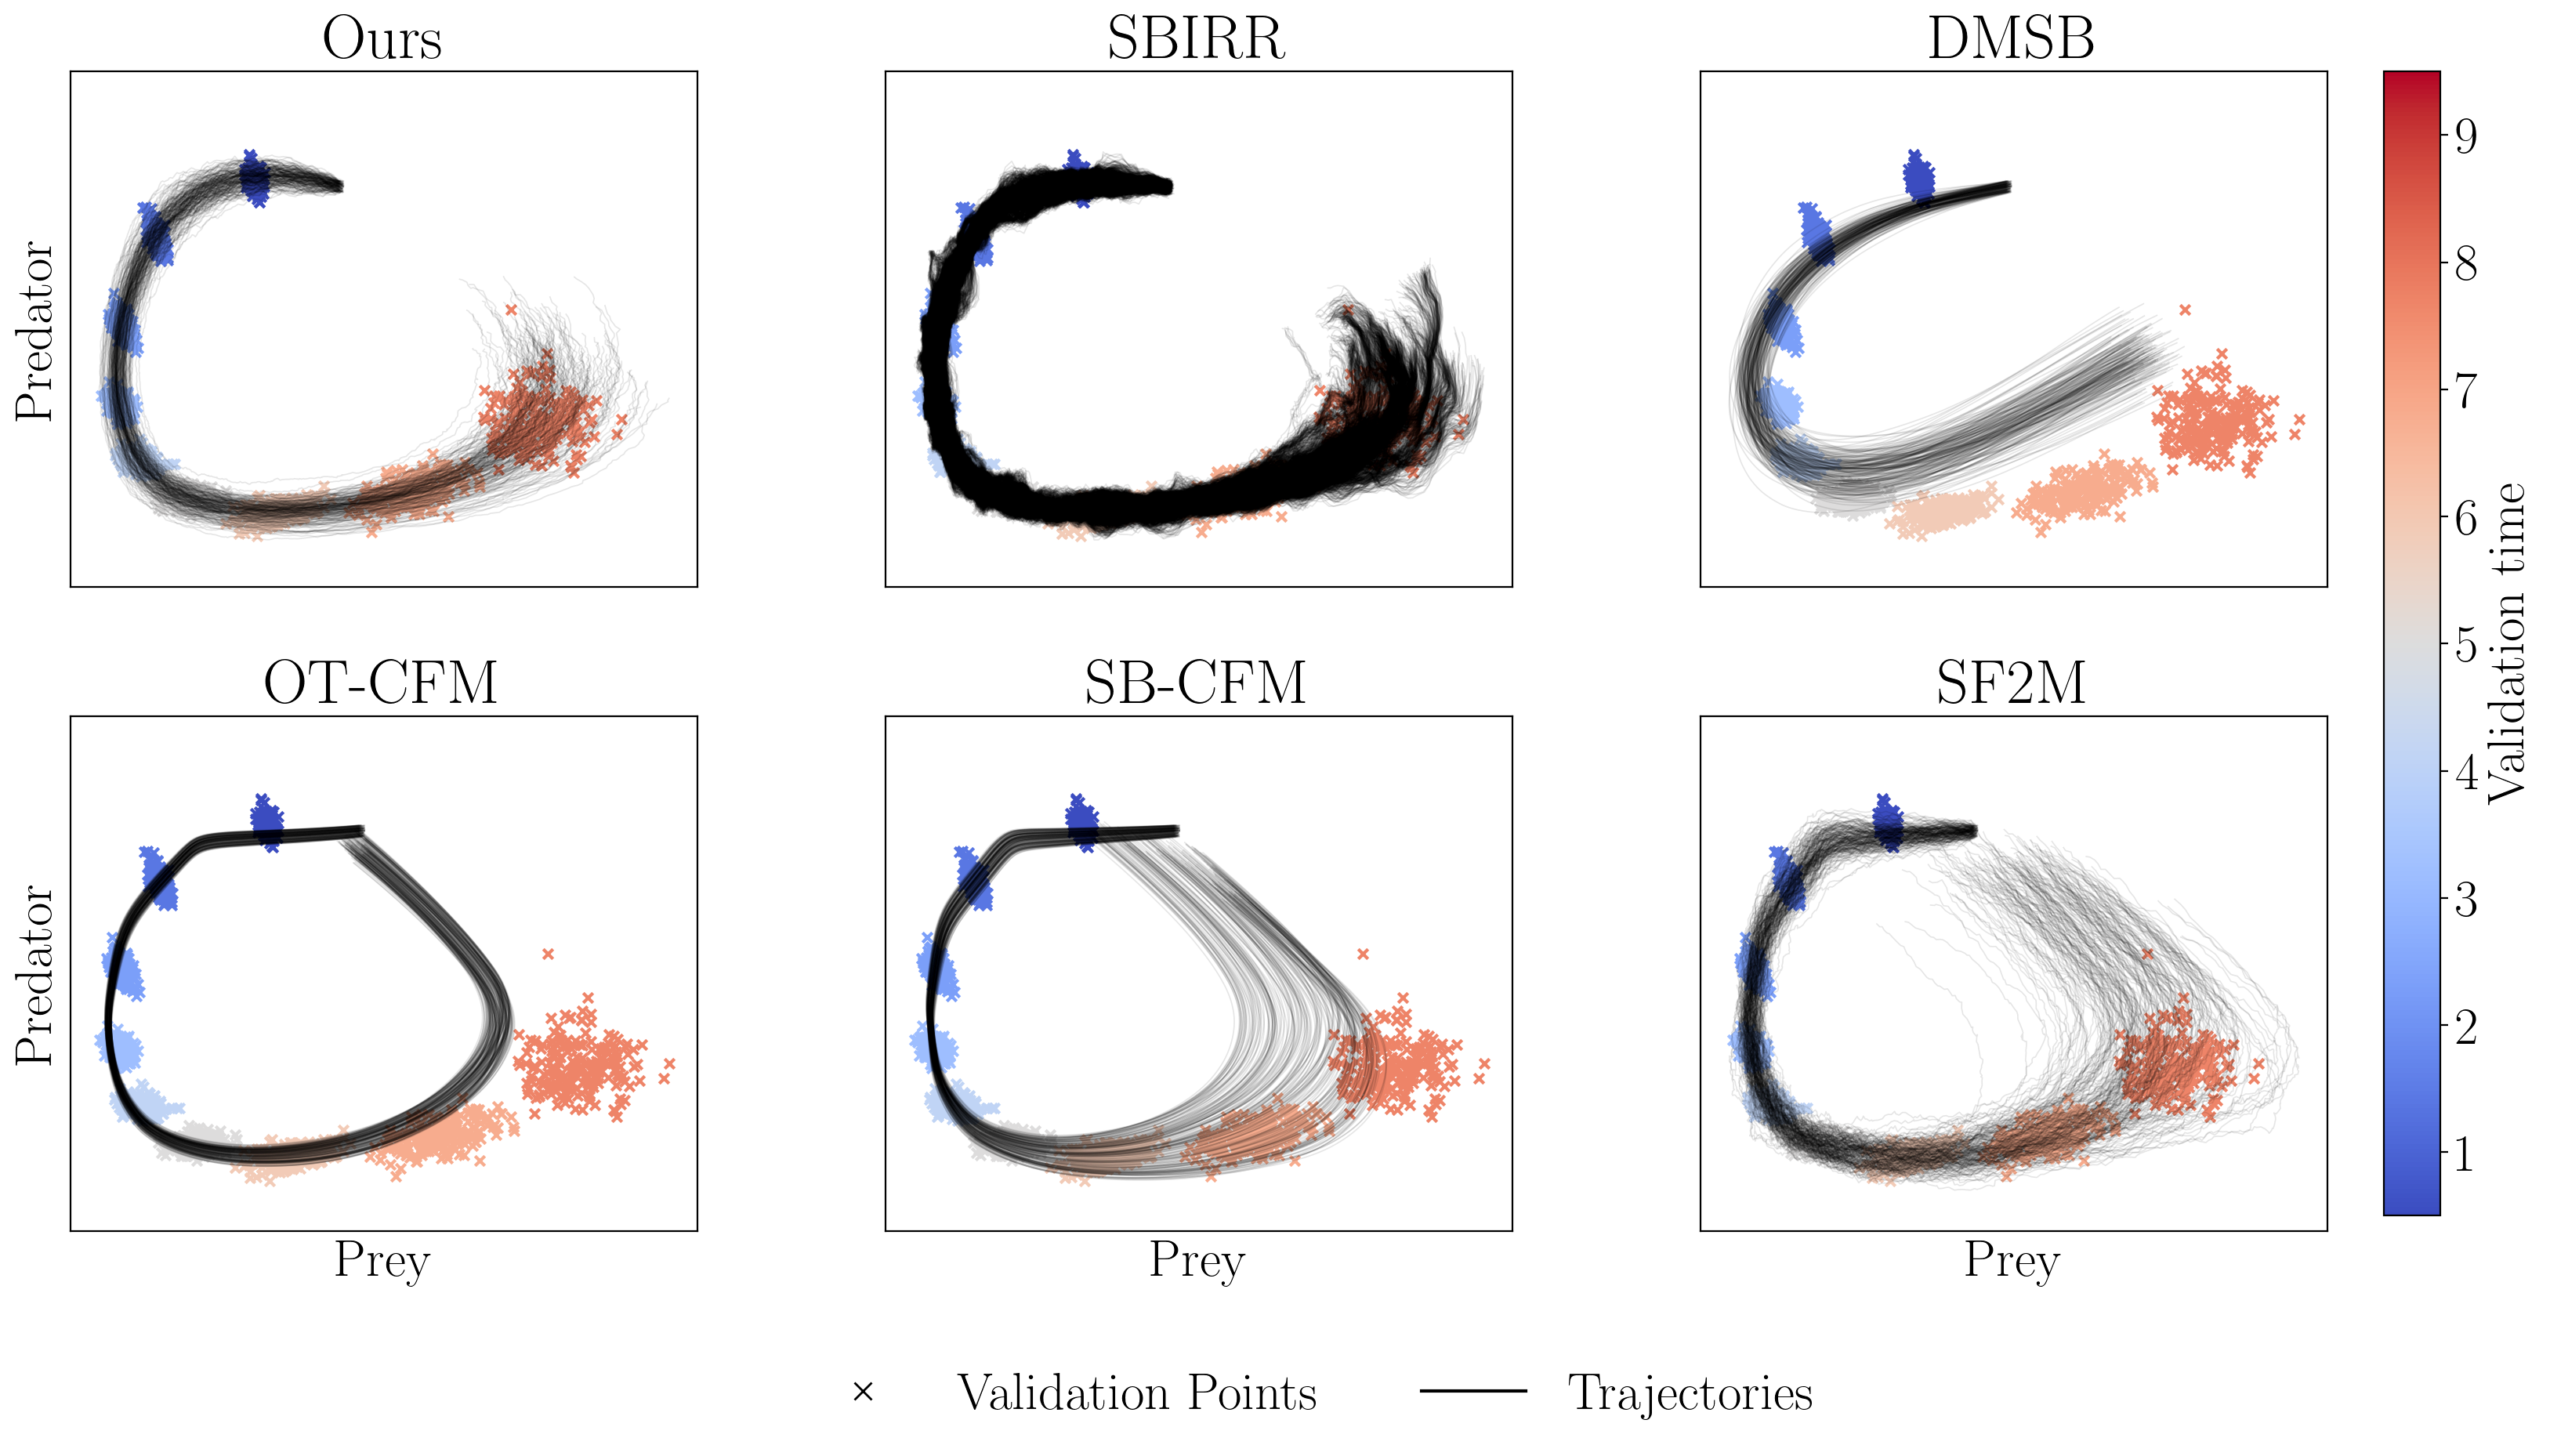
\includegraphics[width=\linewidth]{Figs/LV_interpolationing.png}
    \caption{LV interpolation}
    \label{fig:lv-appendix-parametric-interpol}
\end{figure}

\begin{figure}[!ht]
    \centering
    \includegraphics[width=\linewidth]{Figs/LV_classic_interpolation_metric.pdf}
    \caption{LV interpolation metrics}
    \label{fig:lv-metrics-interpol}
\end{figure}


\begin{table}[ht]
\caption{MMD at each validation point for Lotka-Volterra.}
\centering
\makebox[0pt][c]{
\small
\begin{tabular}{lrrrrrr}
\toprule
Time & Ours & \texttt{SBIRR} & \texttt{DMSB} & \texttt{OT-CFM} & \texttt{SB-CFM} & \texttt{SF2M} \\\midrule
0.5 & \cellcolor{green!25}\bm{$0.010\pm{ 0.003}$} & $0.016\pm{ 0.010}$ & $2.173\pm{ 0.238}$ & $0.188\pm{ 0.038}$ & $0.187\pm{ 0.027}$ & $0.172\pm{ 0.026}$ \\
1.5 & \cellcolor{green!25}\bm{$0.006\pm{ 0.004}$} & $0.014\pm{ 0.013}$ & $2.170\pm{ 0.871}$ & $0.197\pm{ 0.054}$ & $0.203\pm{ 0.053}$ & $0.190\pm{ 0.030}$ \\
2.5 & \cellcolor{green!25}\bm{$0.005\pm{ 0.003}$} & $0.011\pm{ 0.007}$ & $0.462\pm{ 0.364}$ & $0.366\pm{ 0.066}$ & $0.399\pm{ 0.102}$ & $0.348\pm{ 0.045}$ \\
3.5 & $0.015\pm{ 0.007}$ & \cellcolor{green!25}\bm{$0.007\pm{ 0.005}$} & $2.277\pm{ 1.094}$ & $0.501\pm{ 0.233}$ & $0.438\pm{ 0.146}$ & $0.433\pm{ 0.091}$ \\
4.5 & \cellcolor{green!25}\bm{$0.010\pm{ 0.007}$} & \cellcolor{green!25}$0.015\pm{ 0.016}$ & $2.974\pm{ 0.979}$ & $1.254\pm{ 0.838}$ & $0.850\pm{ 0.392}$ & $1.126\pm{ 0.338}$ \\
5.5 & \cellcolor{green!25}\bm{$0.017\pm{ 0.010}$} & \cellcolor{green!25}$0.019\pm{ 0.006}$ & $2.814\pm{ 0.969}$ & $3.913\pm{ 1.804}$ & $2.858\pm{ 1.257}$ & $3.389\pm{ 0.689}$ \\
6.5 & \cellcolor{green!25}\bm{$0.014\pm{ 0.009}$} & \cellcolor{green!25}$0.020\pm{ 0.012}$ & $3.578\pm{ 1.221}$ & $6.755\pm{ 1.498}$ & $5.059\pm{ 1.679}$ & $5.010\pm{ 0.702}$ \\
7.5 & \cellcolor{green!25}\bm{$0.016\pm{ 0.021}$} & $0.080\pm{ 0.058}$ & $6.330\pm{ 0.995}$ & $6.322\pm{ 1.470}$ & $4.006\pm{ 1.880}$ & $4.044\pm{ 0.869}$ \\
8.5 & \cellcolor{green!25}\bm{$0.020\pm{ 0.015}$} & $0.249\pm{ 0.084}$ & $7.066\pm{ 0.778}$ & $5.970\pm{ 1.508}$ & $4.895\pm{ 1.414}$ & $3.787\pm{ 0.502}$ \\
\bottomrule
\end{tabular}}
\label{tab:lv-mmd}
\end{table}


\begin{table}[ht]
\caption{EMD at each validation point for Lotka-Volterra.}
\centering
\makebox[0pt][c]{
\small
\begin{tabular}{lrrrrrr}
\toprule
Time & Ours & \texttt{SBIRR} & \texttt{DMSB} & \texttt{OT-CFM} & \texttt{SB-CFM} & \texttt{SF2M} \\\midrule
0.5 & \cellcolor{green!25}\bm{$0.040\pm{ 0.005}$} & $0.050\pm{ 0.011}$ & $0.503\pm{ 0.031}$ & $0.147\pm{ 0.014}$ & $0.145\pm{ 0.010}$ & $0.139\pm{ 0.010}$ \\
1.5 & \cellcolor{green!25}\bm{$0.037\pm{ 0.006}$} & $0.053\pm{ 0.012}$ & $0.503\pm{ 0.119}$ & $0.157\pm{ 0.017}$ & $0.155\pm{ 0.017}$ & $0.149\pm{ 0.010}$ \\
2.5 & \cellcolor{green!25}\bm{$0.036\pm{ 0.005}$} & $0.050\pm{ 0.009}$ & $0.215\pm{ 0.088}$ & $0.207\pm{ 0.018}$ & $0.213\pm{ 0.026}$ & $0.198\pm{ 0.012}$ \\
3.5 & \cellcolor{green!25}$0.052\pm{ 0.006}$ & \cellcolor{green!25}\bm{$0.049\pm{ 0.007}$} & $0.529\pm{ 0.157}$ & $0.236\pm{ 0.050}$ & $0.222\pm{ 0.036}$ & $0.223\pm{ 0.023}$ \\
4.5 & \cellcolor{green!25}\bm{$0.049\pm{ 0.008}$} & $0.073\pm{ 0.014}$ & $0.647\pm{ 0.135}$ & $0.382\pm{ 0.133}$ & $0.321\pm{ 0.072}$ & $0.383\pm{ 0.069}$ \\
5.5 & \cellcolor{green!25}\bm{$0.065\pm{ 0.012}$} & \cellcolor{green!25}$0.076\pm{ 0.010}$ & $0.653\pm{ 0.134}$ & $0.795\pm{ 0.254}$ & $0.654\pm{ 0.188}$ & $0.841\pm{ 0.173}$ \\
6.5 & \cellcolor{green!25}\bm{$0.077\pm{ 0.012}$} & \cellcolor{green!25}$0.086\pm{ 0.014}$ & $0.829\pm{ 0.177}$ & $1.537\pm{ 0.479}$ & $1.244\pm{ 0.439}$ & $1.652\pm{ 0.376}$ \\
7.5 & \cellcolor{green!25}\bm{$0.096\pm{ 0.025}$} & $0.148\pm{ 0.040}$ & $1.510\pm{ 0.241}$ & $1.705\pm{ 0.586}$ & $1.246\pm{ 0.594}$ & $1.751\pm{ 0.477}$ \\
8.5 & \cellcolor{green!25}\bm{$0.124\pm{ 0.019}$} & $0.283\pm{ 0.037}$ & $1.983\pm{ 0.323}$ & $1.511\pm{ 0.454}$ & $1.825\pm{ 0.662}$ & $1.594\pm{ 0.298}$ \\
\bottomrule
\end{tabular}}
\label{tab:lv-emd}
\end{table}


\clearpage



\subsection{mRNA-only repressilator with parametric family}
\label{app:repr-app-parametric}

\subsubsection{Experiment setup}
\label{app:repr-setup-parametric}
The repressilator is a synthetic genetic circuit designed to function as a biological oscillator, producing sustained periodic fluctuations in the concentrations of its components. It consists of a network of three genes arranged in a cyclic inhibitory loop: each gene encodes a protein that suppresses the expression of the next, with the last gene repressing the first, completing the feedback cycle.

The system’s dynamics can be described by the following stochastic differential equations (SDEs):
\begin{align}
\label{eq:repr-family}
    dX_1 &= \frac{\beta}{1+(X_3/k)^n} - \gamma X_1 + \sigma X_1 dW_1, \nonumber \\
    dX_2 &= \frac{\beta}{1+(X_1/k)^n} - \gamma X_2 + \sigma X_2 dW_2, \\
    dX_3 &= \frac{\beta}{1+(X_2/k)^n} - \gamma X_3 + \sigma X_3 dW_3, \nonumber
\end{align}
where $[dW_1, dW_2, dW_3]$ represents a three-dimensional Brownian motion. The inhibitory structure of the system is evident from the drift terms, which describe how each gene’s expression is repressed by another in the cycle. For our simulations, we set the parameters to $\beta = 10$, $n = 3$, $k = 1$, $\gamma = 1$, and $\sigma = 0.02$. The initial conditions are sampled from uniform distributions: $X_1, X_2 \sim U(1,1.1)$ and $X_3 \sim U(2,2.1)$. To simulate the system, we numerically integrate the SDEs over 19 discrete time points, with sampling rate 0.5 with the Euler-Maruyama scheme(implemented via the \texttt{torchsde} Python package) with 200 samples at each step. Out of these 19 time steps, we use the 10 odd-numbered time steps as training data. The 9 even-numbered time steps are held out for evaluating interpolation performance. To assess forecasting, we simulate one additional time step beyond the final snapshot, using a larger time increment of 1.0, and hold it out as the test point.


\subsubsection{Model family choice}
\label{app:repr_implementation-parametric}
For this experiment, we have access to the data-generating process, as described in \cref{eq:repr-family}. Therefore, we pick as a model family the set of SDEs that satisfy this system of equations, \cref{eq:repr-family}. The learning process involves optimizing the parameters using gradient descent, with a learning rate of 0.05 over 500 epochs. We choose this number of epochs such that in the last 20 epochs $R^2$ increases by less than 0.01. We implemented the model family as a Python class using in the \texttt{torchsde} \citep{li2020scalable} module.

\subsubsection{Forecasting results.}
\label{app:repr-forecasting-parametric}
In this section we further discuss results for the repressilator experiment with parametric model family. In particular, we analyze the EMD and MMD in \cref{tab:repr-param}.

\begin{figure}[t!]
    \centering
    \includegraphics[width=\linewidth]{Figs/Repressilator_forecasting.pdf}
    \caption{Forecasting task for the repressilator system with parametric model family. }
    \label{fig:repr-parametric-forecast}
\end{figure}

\begin{figure}[t!]
    \centering
    \includegraphics[width=\linewidth]{Figs/Repressilator_appendix_diff_arrows.pdf}
    \caption{Experimental results for the repressilator system using parametric model as model family.\textit{Top row}: forecast prediction task. A method is successful if the forecast predicted points (in red) match the red points in the ground truth figure. \textit{Middle row:} ground truth vector field (left) and reconstructed vector fields with the three methods. \textit{Bottom row:} Difference between reconstructed vector fields and ground truth. For each point of interest on the grid, we represent the difference between the two vectors with an arrow and color it according to the magnitude of the difference (colorbar to the right).}
    \label{fig:repr-appendix-parametric}
\end{figure}

\begin{table}[ht!]
    \centering
    \caption{Evaluation metric for repressilator when using the parametric model (mean(sd)). Drift was evaluated using MSE on a grid.}
    \begin{tabular}{lccc}
    \hline
    &     & Repressilator (parametric) & \\
    Metric     &  Ours & \texttt{SBIRR-ref} & \texttt{SB-forward} \\
    \hline
    Forecast-MMD &  \cellcolor{green!25}\textbf{0.072 (0.080)} &2.06 (1.34)& 2.09 (0.74) \\
    Forecast-EMD &  \cellcolor{green!25}\textbf{0.19 (0.075)} &1.55 (0.79)& 1.39 (0.62) \\
    Drift & \cellcolor{green!25}\textbf{0.027 (0.063)} & 1.71 (0.20)& 12.9 (0.21) \\
    \hline
    \end{tabular}
    
    \label{tab:repr-param}
\end{table}

In the first row of \cref{tab:repr-param}, we see that for the forecasting task, our method achieves a much lower MMD compared to the two baselines. This quantitatively supports the visual intuition from \cref{fig:repr-parametric-forecast}, where our approach more accurately captures the underlying distribution of the data. In the second row, we see that also using EMD our method significantly outperforms all the baselines. 

\subsubsection{Vector field reconstruction results.}
\label{app:repr-vector-parametric}

In the third row of \cref{tab:repr-param}, we observe that the MSE for the vector field reconstruction task is significantly lower for our method, indicating superior performance in recovering the true dynamics. This is further corroborated by the visualizations in \cref{fig:repr-appendix-parametric}: in the middle row, our reconstructed vector field closely resembles the ground truth, whereas \texttt{SBIRR-ref} exhibits small but notable deviations, and \texttt{SB-forward} fails both in magnitude and direction. The bottom row further reinforces this conclusion, showing that the magnitude of the differences between the reconstructed and true vector fields is substantially larger for the two baselines compared to our method (for which is very close to 0 everywhere on the grid).

\subsubsection{Interpolation results}
\label{app:repr-interpol-parametric}

We next assess interpolation performance for the parametric model, again comparing inferred trajectories to held-out snapshots with MMD and EMD. Visual inspection of \cref{fig:repr-appendix-parametric-interpol} shows that our method interpolates all the validation snapshots very closely, understanding the periodic behavior of this system. \texttt{SBIRR} yields a qualitatively similar plot with more noisy trajectories, while \texttt{DMSB}, \texttt{OT-CFM}, \texttt{SB-CFM}, and \texttt{SF2M} provide poor interpolations --- \texttt{OT-CFM} fails because they are just pairwise interpolation methods and so they “connect” training points, missing the long-term behavior of the system; \texttt{DMSB}, \texttt{SB-CFM} , and \texttt{SF2M} fail because they start drifting outward and end up very far from the actual validation points.  

The metric curves in \cref{fig:repr-metric-interpol} and tables \cref{tab:repr-classic-mmd}–\cref{tab:repr-classic-emd} corroborate these impressions. Across all validation times, our method always achieves the lowest MMD and EMD, whereas the second best method (\texttt{SBIRR} ) is comparable to ours only on one validation time. All the other baselines achieve worse performance. We note that in  \cref{fig:repr-metric-interpol} we set the y-axis limit to 5 to show meaningful comparisons. We did this since \texttt{SF2M} ’s EMD explodes after time 5.5 --- peaking at $\approx 138$ at time 8.5 --- signalling complete geometric mismatch with the target distribution. We also refrain from highlighting the \texttt{SF2M}  cell in green, despite it formally satisfying the coloring criterion. This is because the overlap with the best-performing method arises primarily from \texttt{SF2M} 's extremely large mean and standard deviation, rather than from a meaningful proximity in performance.

\begin{figure}[!ht]
    \centering
    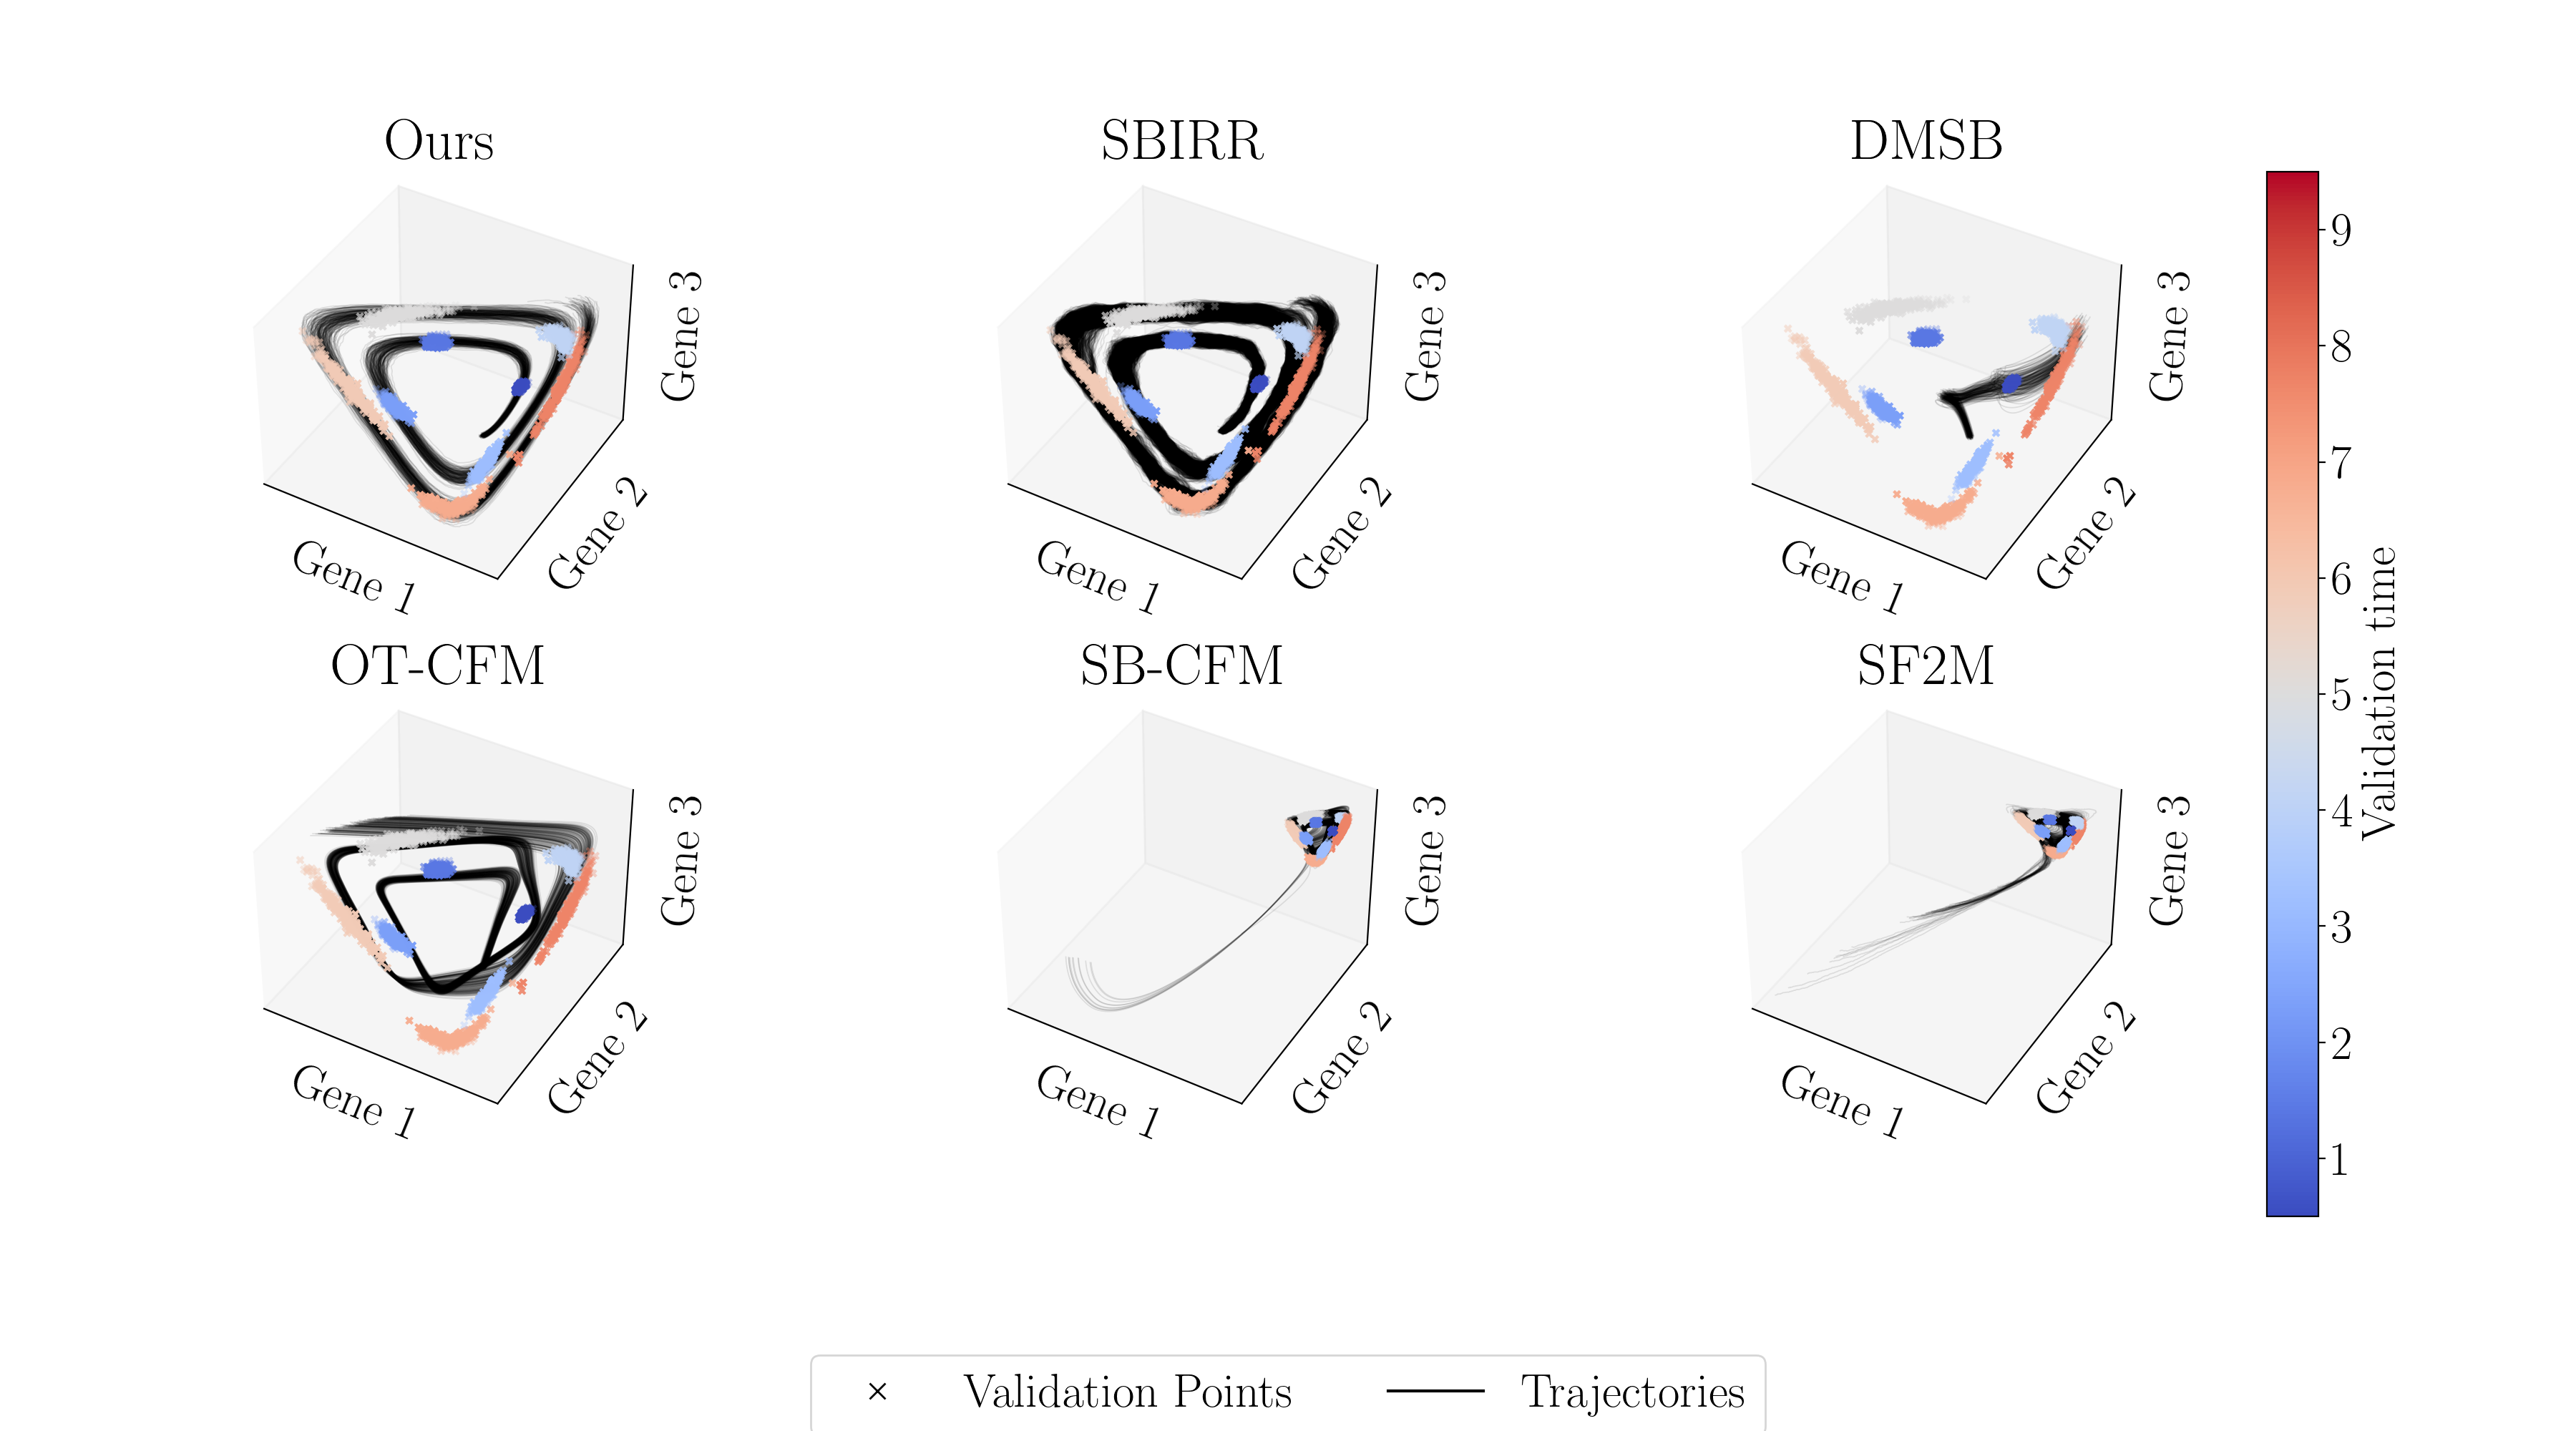
\includegraphics[width=\linewidth]{Figs/Repressilator_interpolationing.png}
    
    \caption{Parametric interpolation}
    \label{fig:repr-appendix-parametric-interpol}
\end{figure}

\begin{figure}[!ht]
    \centering
    \includegraphics[width=\linewidth]{Figs/Repressilator_classic_interpolation_metric.pdf}
    \caption{Parametric interpolation metric}
    \label{fig:repr-metric-interpol}
\end{figure}

\begin{table}[ht]
\caption{MMD at each validation point  for Repressilator parametric.}
\centering
\makebox[0pt][c]{
\small
\begin{tabular}{lrrrrrr}
\toprule
Time & Ours & \texttt{SBIRR} & \texttt{DMSB} & \texttt{OT-CFM} & \texttt{SB-CFM} & \texttt{SF2M} \\\midrule
0.5 & \cellcolor{green!25}\bm{$0.022\pm{ 0.004}$} & $0.151\pm{ 0.061}$ & $8.104\pm{ 0.230}$ & $2.767\pm{ 0.137}$ & $2.768\pm{ 0.162}$ & $2.639\pm{ 0.137}$ \\
1.5 & $0.070\pm{ 0.020}$ & \cellcolor{green!25}\bm{$0.037\pm{ 0.024}$} & $7.324\pm{ 0.625}$ & $1.280\pm{ 0.469}$ & $1.103\pm{ 0.498}$ & $1.267\pm{ 0.370}$ \\
2.5 & \cellcolor{green!25}\bm{$0.019\pm{ 0.009}$} & $0.120\pm{ 0.044}$ & $6.438\pm{ 0.823}$ & $5.468\pm{ 1.053}$ & $3.876\pm{ 0.687}$ & $3.661\pm{ 0.531}$ \\
3.5 & \cellcolor{green!25}\bm{$0.059\pm{ 0.036}$} & $0.148\pm{ 0.047}$ & $8.262\pm{ 0.819}$ & $6.943\pm{ 1.067}$ & $5.393\pm{ 1.852}$ & $4.792\pm{ 0.985}$ \\
4.5 & \cellcolor{green!25}\bm{$0.025\pm{ 0.031}$} & $0.150\pm{ 0.054}$ & $8.929\pm{ 0.245}$ & $4.600\pm{ 1.465}$ & $2.969\pm{ 1.475}$ & $3.633\pm{ 0.684}$ \\
5.5 & \cellcolor{green!25}\bm{$0.060\pm{ 0.029}$} & $0.094\pm{ 0.021}$ & $8.124\pm{ 0.204}$ & $3.818\pm{ 1.405}$ & $2.385\pm{ 1.362}$ & $2.757\pm{ 0.528}$ \\
6.5 & \cellcolor{green!25}\bm{$0.032\pm{ 0.019}$} & $0.214\pm{ 0.054}$ & $7.610\pm{ 0.124}$ & $5.015\pm{ 1.699}$ & $2.926\pm{ 1.436}$ & $3.134\pm{ 0.463}$ \\
7.5 & \cellcolor{green!25}\bm{$0.020\pm{ 0.013}$} & $0.379\pm{ 0.058}$ & $8.404\pm{ 0.130}$ & $6.561\pm{ 1.667}$ & $5.488\pm{ 1.984}$ & $4.473\pm{ 0.695}$ \\
8.5 & \cellcolor{green!25}\bm{$0.053\pm{ 0.057}$} & \cellcolor{green!25}$0.108\pm{ 0.030}$ & $2.225\pm{ 1.179}$ & $5.297\pm{ 1.601}$ & $4.595\pm{ 0.725}$ & $3.589\pm{ 0.616}$ \\
\bottomrule
\end{tabular}}
\label{tab:repr-classic-mmd}
\end{table}


\begin{table}[ht]
\caption{EMD at each validation point for Repressilator parametric.}
\centering
\makebox[0pt][c]{
\small
\begin{tabular}{lrrrrrr}
\toprule
Time & Ours & \texttt{SBIRR} & \texttt{DMSB} & \texttt{OT-CFM} & \texttt{SB-CFM} & \texttt{SF2M} \\\midrule
0.5 & \cellcolor{green!25}\bm{$0.052\pm{ 0.004}$} & $0.129\pm{ 0.025}$ & $1.317\pm{ 0.053}$ & $0.578\pm{ 0.017}$ & $0.581\pm{ 0.022}$ & $0.581\pm{ 0.021}$ \\
1.5 & \cellcolor{green!25}$0.091\pm{ 0.013}$ & \cellcolor{green!25}\bm{$0.080\pm{ 0.017}$} & $1.192\pm{ 0.104}$ & $0.384\pm{ 0.075}$ & $0.436\pm{ 0.165}$ & $0.569\pm{ 0.143}$ \\
2.5 & \cellcolor{green!25}\bm{$0.061\pm{ 0.009}$} & $0.128\pm{ 0.021}$ & $1.095\pm{ 0.131}$ & $0.985\pm{ 0.145}$ & $0.920\pm{ 0.164}$ & $1.023\pm{ 0.152}$ \\
3.5 & \cellcolor{green!25}\bm{$0.102\pm{ 0.023}$} & $0.157\pm{ 0.019}$ & $1.762\pm{ 0.330}$ & $1.424\pm{ 0.166}$ & $1.176\pm{ 0.229}$ & $1.515\pm{ 0.416}$ \\
4.5 & \cellcolor{green!25}\bm{$0.070\pm{ 0.021}$} & $0.153\pm{ 0.018}$ & $2.086\pm{ 0.348}$ & $1.104\pm{ 0.316}$ & $0.984\pm{ 0.571}$ & $2.618\pm{ 1.923}$ \\
5.5 & \cellcolor{green!25}\bm{$0.120\pm{ 0.025}$} & $0.170\pm{ 0.020}$ & $2.428\pm{ 0.409}$ & $1.193\pm{ 0.312}$ & $1.194\pm{ 0.986}$ & $5.505\pm{ 7.561}$ \\
6.5 & \cellcolor{green!25}\bm{$0.118\pm{ 0.028}$} & $0.238\pm{ 0.032}$ & $3.006\pm{ 0.279}$ & $2.068\pm{ 0.502}$ & $1.765\pm{ 1.185}$ & $14.974\pm{ 27.778}$ \\
7.5 & \cellcolor{green!25}\bm{$0.099\pm{ 0.018}$} & $0.257\pm{ 0.020}$ & $3.270\pm{ 0.310}$ & $2.556\pm{ 0.842}$ & $2.306\pm{ 1.469}$ & $44.051\pm{ 96.243}$ \\
8.5 & \cellcolor{green!25}\bm{$0.152\pm{ 0.061}$} & \cellcolor{green!25}$0.198\pm{ 0.021}$ & $0.828\pm{ 0.266}$ & $2.011\pm{ 0.534}$ & $3.345\pm{ 2.295}$ & $137.973\pm{ 328.155}$ \\
\bottomrule
\end{tabular}}
\label{tab:repr-classic-emd}
\end{table}


\clearpage

\subsection{mRNA-only repressilator with semiparametric family}
\label{app:repr-app-semiparametric}

\subsubsection{Experiment setup}
\label{app:repr-setup-semiparametric}
The experimental setup is the same as the one for the repressilator with the parametric model choice, as discussed in \cref{app:repr-setup-parametric}.

\subsubsection{Model family choice}
\label{app:repr_implementation-semiparametric}
In this experiment, we do not assume that we know the full functional form as in \cref{eq:repr-family}, but only up to an unknown activation function $f_{\bm \theta} : \R_{+}^{3}\to [0,1]^3$, that encodes the regulation among the three genes. In particular, we consider the following model:
\begin{equation}
    d\responseat{\timet}=\bm{M}f_{\bm \theta}(\responseat{\timet})-\bm{L} \responseat{\timet}+\bm{G} \diag(\responseat{\timet})d\bm{W}_{\timet}
    \label{eq:mlpactive}
\end{equation}
where $\bm{M}$ is a diagonal matrix of (positive) maximum production rate, $\bm{L}$ is a diagonal matrix of (positive) degradation rate, $\bm{G}$ is a diagonal matrix of (positive) volatilities, all unknown (parameterized by their logarithm). We also parameterize the activation function using an MLP with three hidden layers of [32, 64, 32] hidden neurons each, ReLU activation, and one final sigmoid layer. 

\subsubsection{Forecasting results.}
\label{app:repr-forecasting-semiparametric}
For what concerns the experiment with the semiparametric model family, we can see in the first row of \cref{tab:repr-mlp} that also with this model our method achieves a substantially lower MMD compared to the two baselines. This aligns with the visual evidence from \cref{fig:repr-main} in the main text (top row), where our method’s predicted points (in red) more closely match the ground truth. In the second row of \cref{tab:repr-mlp}, we see that EMD results are aligned with the MMD ones. 

\subsubsection{Vector field reconstruction results.}
\label{app:repr-vector-semiparametric}

In the third row of \cref{tab:repr-mlp}, we see that for this model choice our method and \texttt{SBIRR-ref} achieve similar results, whereas \texttt{SB-forward} exhibits much higher MSE. \Cref{fig:repr-appendix-semiparametric} confirms this intuition: our reconstructed vector field and the one for \texttt{SBIRR-ref} are quite similar and not too different from the ground truth, whereas \texttt{SB-forward} performs particularly poorly, failing to recover both the direction and magnitude of the vector field. 

\begin{table}[ht!]
    \centering
    \caption{Evaluation metric for Repressilator using MLP activation function (mean(sd)). Drift was evaluated using MSE on a grid, while forecast was evaluated using MMD with RBF kernel and length scale 1 as well as EMD.}
    \begin{tabular}{lccc}
    \hline
    &     & Repressilator (semiparametric) & \\
    Metric     &  Ours & \texttt{SBIRR-ref} & \texttt{SB-forward} \\
    \hline
    Forecast-MMD & \cellcolor{green!25}\textbf{0.32 (0.15)}& 1.46 (0.55) & 5.26 (1.66) \\
    Forecast-EMD & \cellcolor{green!25}\textbf{0.35 (0.091)}& 1.18 (0.44) & 1.16 (0.33) \\
    Drift & \cellcolor{green!25}\textbf{6.25 (0.37)} & \cellcolor{green!25}\textbf{7.85 (1.85)} & 12.00 (0.74)  \\
    \hline
    \end{tabular}
    \label{tab:repr-mlp}
\end{table}


\begin{figure}[h!]
    \centering
    \includegraphics[width=\linewidth]{Figs/mlp_Repressilator_appendix_diff_arrows.pdf}
    \caption{Experimental results for the repressilator system using semiparametric model as model family. \textit{Top row}: forecast prediction task. A method is successful if the forecast predicted points (in red) match the red points in the ground truth figure. \textit{Middle row:} ground truth vector field (left) and reconstructed vector fields with the three methods. \textit{Bottom row:} Difference between reconstructed vector fields and ground truth. For each point of interest on the grid, we represent the difference between the two vectors with an arrow and color it according to the magnitude of the difference (colorbar to the right).}
    \label{fig:repr-appendix-semiparametric}
\end{figure}

\subsubsection{Interpolation results}
\label{app:repr-interpol-semiparametric}

We now evaluate interpolation performance in the more realistic semiparametric setting, where neither our method nor \texttt{SBIRR} have access to the true data-generating process. Instead, both methods rely on the same semiparametric reference family from \cref{eq:mlpactive}, introducing a meaningful model mismatch that more closely reflects real-world conditions. As shown in \cref{fig:repr-appendix-semiparametric-interpol}, interpolation quality for our method and \texttt{SBIRR} is very similar to the parametric case, as they both are still very good at interpolating all the validation snapshots. The remaining baselines are not affected by this modeling choice, so the trajectories are exactly as in \cref{fig:repr-appendix-parametric-interpol}.
The quantitative results in \cref{fig:repr-semiparametric-metric-interpol} and tables \cref{tab:repr-mlp-mmd}–\cref{tab:repr-mlp-emd} reinforce these trends. Although all methods exhibit increased error relative to the parametric setting, our method continues to outperform all baselines across nearly all validation times. In terms of MMD, we are the best method at six of nine time points; \texttt{SBIRR} performs similarly at three time points, but is consistently worse on the rest. EMD results are even more decisive: our method achieves the lowest error at every time point. 


\begin{figure}
    \centering
    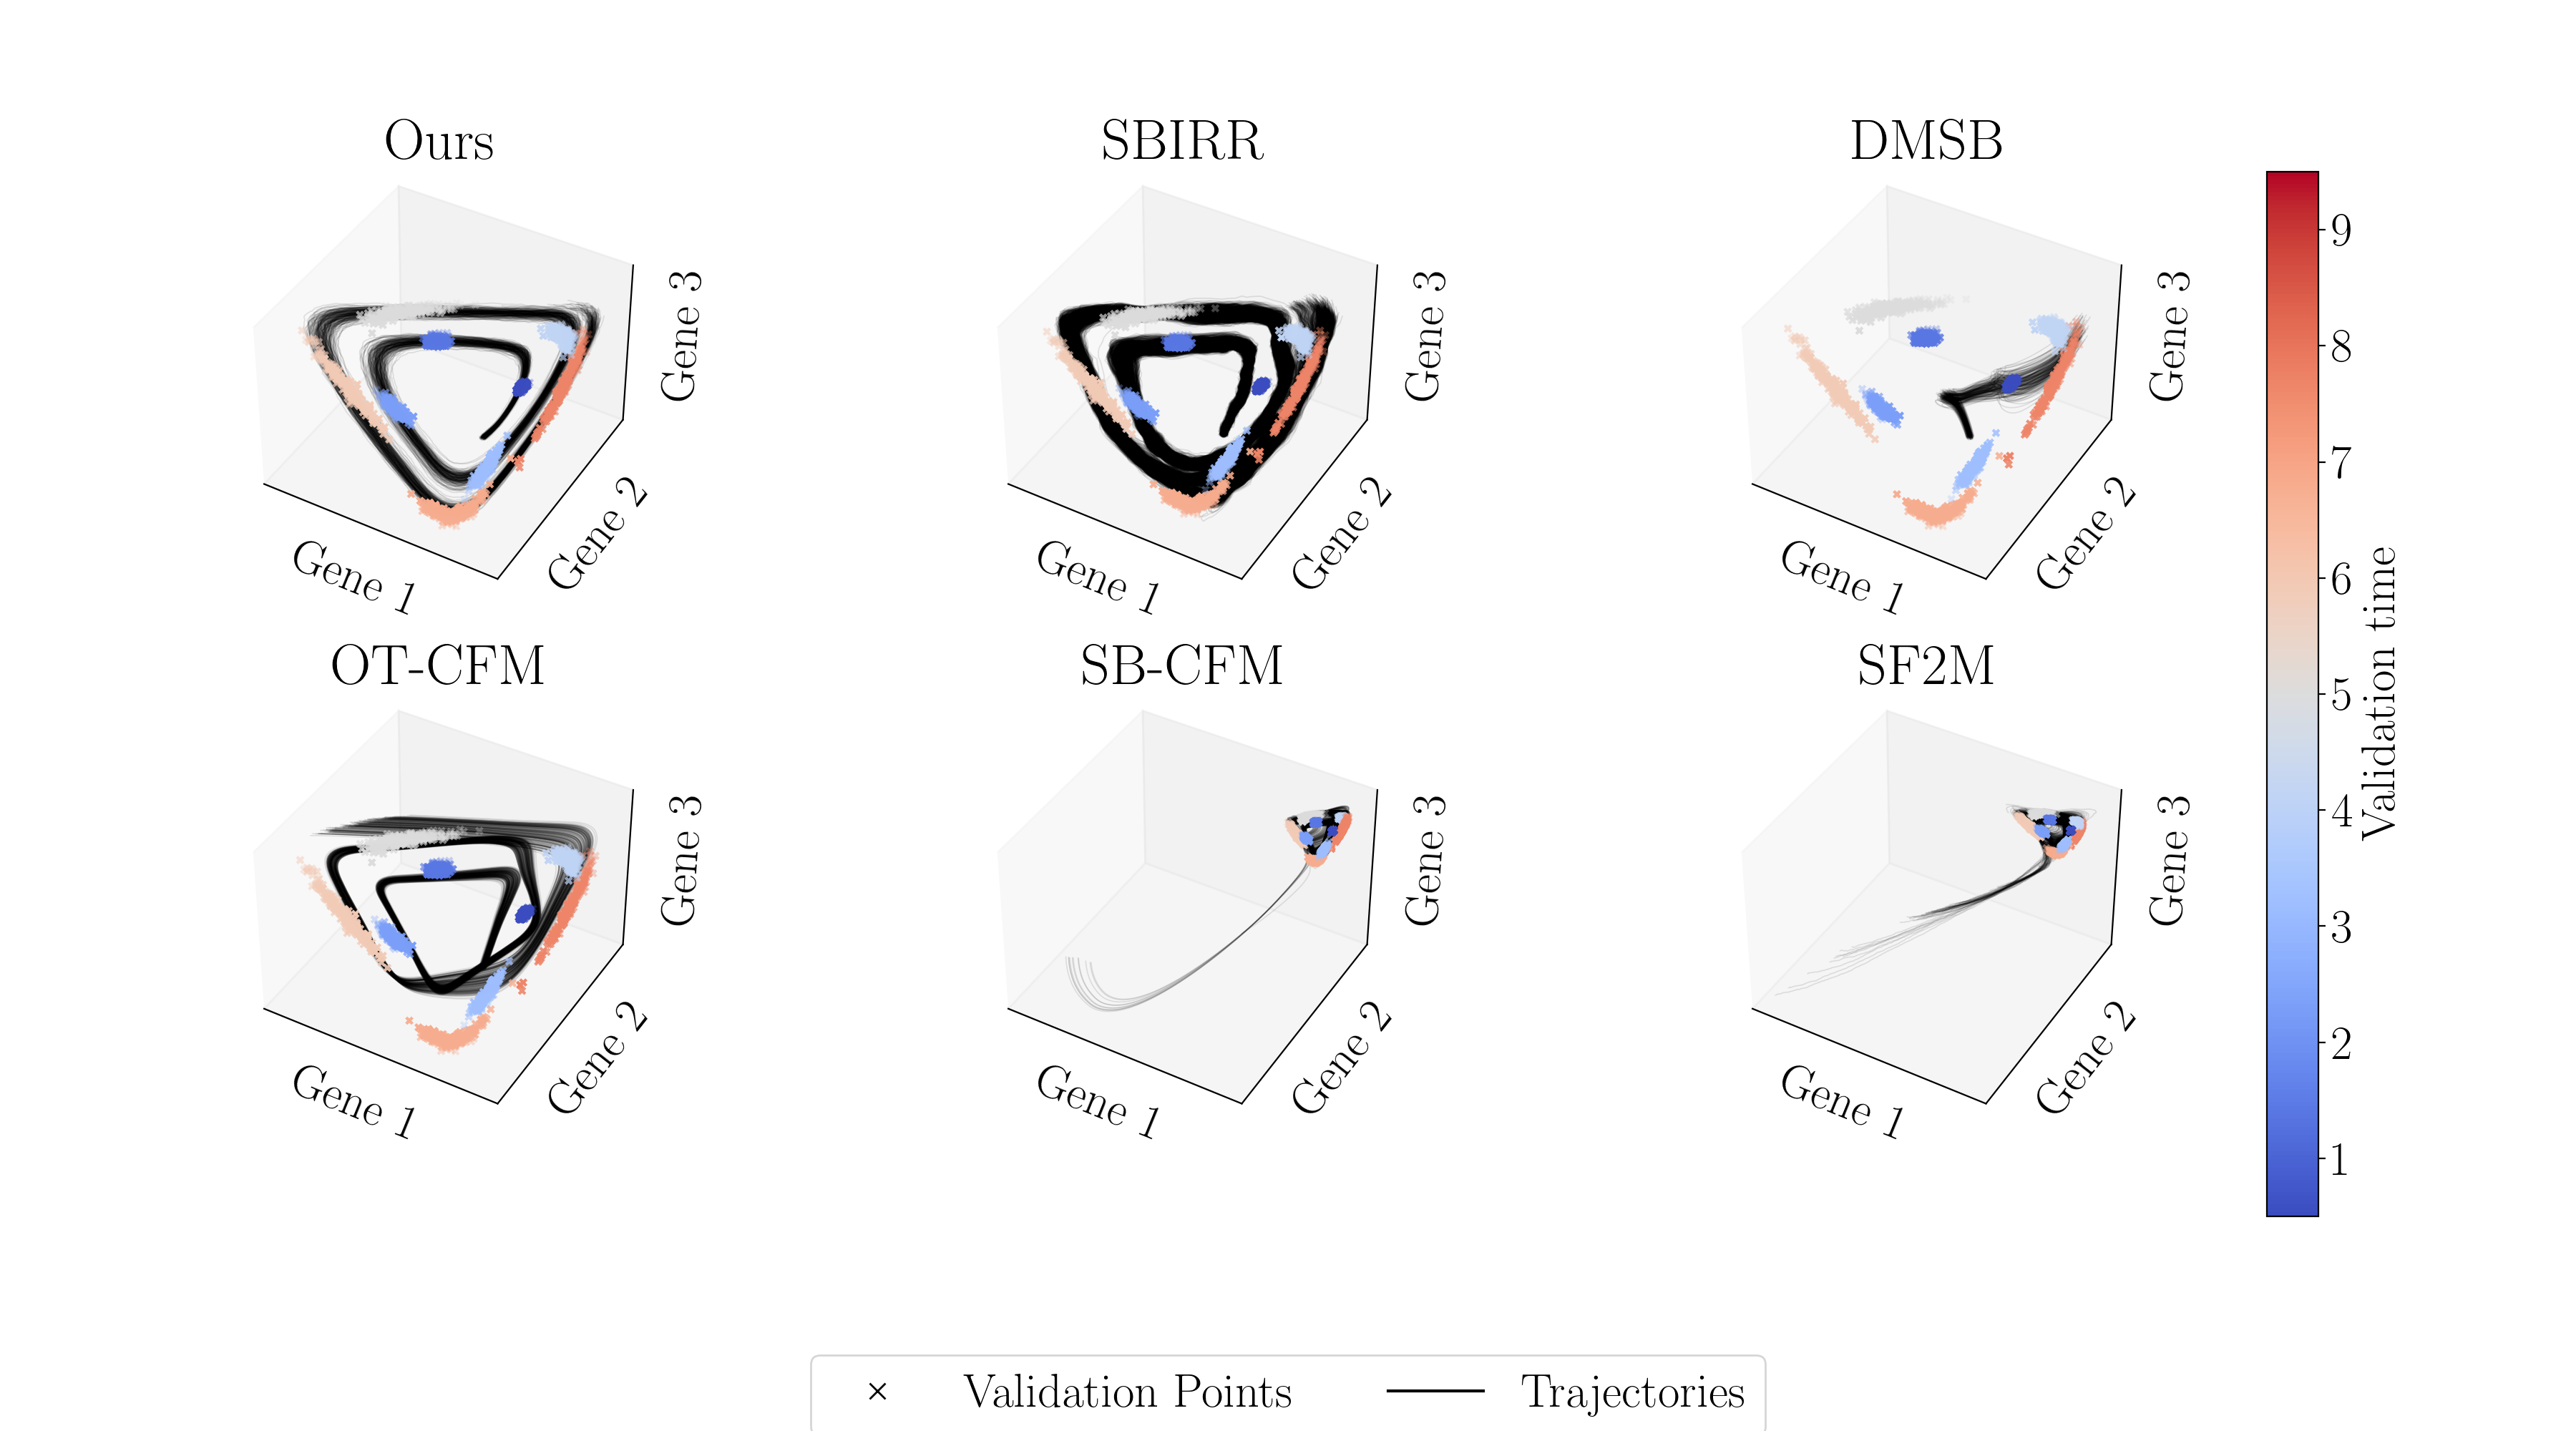
\includegraphics[width=\linewidth]{Figs/mlp_Repressilator_interpolationing.png}
    
    \caption{Semiparametric interpolation of repressilator system.}
    \label{fig:repr-appendix-semiparametric-interpol}
\end{figure}

\begin{figure}
    \centering

    \includegraphics[width=\linewidth]{Figs/Repressilator_mlp_interpolation_metric.pdf}
    \caption{Metrics for Semiparametric interpolation of repressilator system.}
    \label{fig:repr-semiparametric-metric-interpol}
\end{figure}



\begin{table}[ht]
\caption{MMD at each validation point for Repressilator with semiparametric model family.}
\centering
\makebox[0pt][c]{
\small
\begin{tabular}{lrrrrrr}
\toprule
Time & Ours & \texttt{SBIRR} & \texttt{DMSB} & \texttt{OT-CFM} & \texttt{SB-CFM} & \texttt{SF2M} \\\midrule
0.5 & \cellcolor{green!25}\bm{$0.909\pm{ 0.171}$} & $2.422\pm{ 0.470}$ & $8.104\pm{ 0.230}$ & $2.767\pm{ 0.137}$ & $2.768\pm{ 0.162}$ & $2.639\pm{ 0.137}$ \\
1.5 & \cellcolor{green!25}\bm{$0.137\pm{ 0.146}$} & $0.633\pm{ 0.366}$ & $7.324\pm{ 0.625}$ & $1.280\pm{ 0.469}$ & $1.103\pm{ 0.498}$ & $1.267\pm{ 0.370}$ \\
2.5 & \cellcolor{green!25}\bm{$0.274\pm{ 0.277}$} & $0.865\pm{ 0.355}$ & $6.438\pm{ 0.823}$ & $5.468\pm{ 1.053}$ & $3.876\pm{ 0.687}$ & $3.661\pm{ 0.531}$ \\
3.5 & \cellcolor{green!25}\bm{$0.091\pm{ 0.061}$} & $1.529\pm{ 0.515}$ & $8.262\pm{ 0.819}$ & $6.943\pm{ 1.067}$ & $5.393\pm{ 1.852}$ & $4.792\pm{ 0.985}$ \\
4.5 & \cellcolor{green!25}\bm{$0.424\pm{ 0.215}$} & $1.761\pm{ 0.511}$ & $8.929\pm{ 0.245}$ & $4.600\pm{ 1.465}$ & $2.969\pm{ 1.475}$ & $3.633\pm{ 0.684}$ \\
5.5 & \cellcolor{green!25}\bm{$0.061\pm{ 0.031}$} & $0.383\pm{ 0.259}$ & $8.124\pm{ 0.204}$ & $3.818\pm{ 1.405}$ & $2.385\pm{ 1.362}$ & $2.757\pm{ 0.528}$ \\
6.5 & \cellcolor{green!25}$0.455\pm{ 0.174}$ & \cellcolor{green!25}\bm{$0.449\pm{ 0.197}$} & $7.610\pm{ 0.124}$ & $5.015\pm{ 1.699}$ & $2.926\pm{ 1.436}$ & $3.134\pm{ 0.463}$ \\
7.5 & \cellcolor{green!25}\bm{$0.994\pm{ 0.283}$} & $1.663\pm{ 0.474}$ & $8.404\pm{ 0.130}$ & $6.561\pm{ 1.667}$ & $5.488\pm{ 1.984}$ & $4.473\pm{ 0.695}$ \\
8.5 & \cellcolor{green!25}\bm{$0.071\pm{ 0.035}$} & $0.241\pm{ 0.101}$ & $2.225\pm{ 1.179}$ & $5.297\pm{ 1.601}$ & $4.595\pm{ 0.725}$ & $3.589\pm{ 0.616}$ \\
\bottomrule
\end{tabular}}
\label{tab:repr-mlp-mmd}
\end{table}


\begin{table}[ht]
\caption{EMD at each validation point for Repressilator with semiparametric model family.}
\centering
\makebox[0pt][c]{
\small
\begin{tabular}{lrrrrrr}
\toprule
Time & Ours & \texttt{SBIRR} & \texttt{DMSB} & \texttt{OT-CFM} & \texttt{SB-CFM} & \texttt{SF2M} \\\midrule
0.5 & \cellcolor{green!25}\bm{$0.312\pm{ 0.032}$} & $0.533\pm{ 0.061}$ & $1.317\pm{ 0.053}$ & $0.578\pm{ 0.017}$ & $0.581\pm{ 0.022}$ & $0.581\pm{ 0.021}$ \\
1.5 & \cellcolor{green!25}\bm{$0.111\pm{ 0.060}$} & $0.255\pm{ 0.087}$ & $1.192\pm{ 0.104}$ & $0.384\pm{ 0.075}$ & $0.436\pm{ 0.165}$ & $0.569\pm{ 0.143}$ \\
2.5 & \cellcolor{green!25}\bm{$0.167\pm{ 0.082}$} & $0.322\pm{ 0.065}$ & $1.095\pm{ 0.131}$ & $0.985\pm{ 0.145}$ & $0.920\pm{ 0.164}$ & $1.023\pm{ 0.152}$ \\
3.5 & \cellcolor{green!25}\bm{$0.121\pm{ 0.027}$} & $0.493\pm{ 0.091}$ & $1.762\pm{ 0.330}$ & $1.424\pm{ 0.166}$ & $1.176\pm{ 0.229}$ & $1.515\pm{ 0.416}$ \\
4.5 & \cellcolor{green!25}\bm{$0.222\pm{ 0.064}$} & $0.483\pm{ 0.078}$ & $2.086\pm{ 0.348}$ & $1.104\pm{ 0.316}$ & $0.984\pm{ 0.571}$ & $2.618\pm{ 1.923}$ \\
5.5 & \cellcolor{green!25}\bm{$0.122\pm{ 0.023}$} & $0.263\pm{ 0.079}$ & $2.428\pm{ 0.409}$ & $1.193\pm{ 0.312}$ & $1.194\pm{ 0.986}$ & $5.505\pm{ 7.561}$ \\
6.5 & \cellcolor{green!25}\bm{$0.307\pm{ 0.067}$} & \cellcolor{green!25}$0.369\pm{ 0.075}$ & $3.006\pm{ 0.279}$ & $2.068\pm{ 0.502}$ & $1.765\pm{ 1.185}$ & $14.974\pm{ 27.778}$ \\
7.5 & \cellcolor{green!25}\bm{$0.374\pm{ 0.053}$} & $0.542\pm{ 0.081}$ & $3.270\pm{ 0.310}$ & $2.556\pm{ 0.842}$ & $2.306\pm{ 1.469}$ & $44.051\pm{ 96.243}$ \\
8.5 & \cellcolor{green!25}\bm{$0.157\pm{ 0.023}$} & $0.290\pm{ 0.074}$ & $0.828\pm{ 0.266}$ & $2.011\pm{ 0.534}$ & $3.345\pm{ 2.295}$ & $137.973\pm{ 328.155}$ \\
\bottomrule
\end{tabular}}
\label{tab:repr-mlp-emd}

\end{table}


\clearpage


\subsection{mRNA-protein repressilator}
\label{app:repr-app-missing}
\subsubsection{Experiment setup} 
\label{app:repr-missing-setup}
In \cref{app:repr-setup-parametric} we introduced the repressilator system as a system of SDEs governing changes in mRNA concentration. A more complete model for this system takes also into account protein levels. Indeed, each gene produces a protein that represses the next gene's expression, with the last one repressing the first. So proteins play a big role in the repressilator feedback loop. And this is why scientists often consider a more complex version of this system, that evolves according to the following SDEs:
\begin{equation}
    \begin{aligned}
    dX_1&=\alpha + \frac{\beta}{1+(Y_3/k)^n}-\gamma X_1+\sigma X_1dW_1 \\
    dX_2&=\alpha +\frac{\beta}{1+(Y_1/k)^n}-\gamma X_2+\sigma X_2dW_2\\
    dX_3&=\alpha +\frac{\beta}{1+(Y_2/k)^n}-\gamma X_3+\sigma X_2dW_3\\
    dY_1&=\beta_p X_1-\gamma_p Y_1+\sigma Y_1dW_4\\
    dY_2&=\beta_p X_2-\gamma_p Y_2+\sigma Y_2dW_5\\
    dY_3&=\beta_p X_3-\gamma_p Y_3+\sigma Y_3dW_6
\end{aligned}
\label{eq:repr-family-protein}
\end{equation}

where $[dW_1,dW_2,dW_3, dW_4, dW_5, dW_6]$ is a 6D Brownian motion. $X_1,X_2,X_3$ represents the mRNA levels while $Y_1, Y_2, Y_3$ are the corresponding proteins. As explained above, the actual system regulation is now mediated by proteins rather than mRNA themselves. 

To obtain data, we fix the following parameters: $\alpha = 10^{-5}, \beta = 10, n=3, k = 1, \gamma = 1,\beta_p=1, \gamma_p = 1, \sigma = 0.02$. We start the dynamics with initial distribution $X_1, X_2\sim U(1,1.1)$ and $X_3\sim U(2,2.1)$, while $Y_i\sim U(0,0.1)$. We simulate the SDEs for 10 instants of time. 

To simulate the system, we numerically integrate the SDEs over 19 discrete time points, with sampling rate 0.5 with the Euler-Maruyama scheme(implemented via the \texttt{torchsde} Python package) with 200 samples at each step. Out of these 19, we used 10 odd numbered time steps as training and even numbered steps as validation for interpolation task. We further simulate one step further with time increment of 1 to hold out as test point for forecasting. In all these steps we only took $X_i$ as observations

\subsubsection{Model family choice}
\label{app:repr_implementation_protein}
\textbf{Our method.} For this experiment, we have access to the data-generating process, as described in \cref{eq:repr-family-protein}. Therefore, we select our model family to be the set of SDEs that satisfy this system of equations, \cref{eq:repr-family-protein}. We initialize the missing dimensions at all 0. The learning process involves optimizing the parameters using gradient descent, with a learning rate of 0.05 over 500 epochs. We choose this number of epochs such that in the last 20 epochs $R^2$ increases by less than 0.01.

\textbf{A Note on Baselines.} Since the two forecasting baseline methods that we consider cannot handle incomplete state observations we cannot use them to fit \cref{eq:repr-family-protein}. Instead, we fit a simpler mRNA-only model as described in \cref{eq:repr-family}. We do the same for \texttt{SBIRR} in the interpolation experiment. 



\subsubsection{Forecasting results}
\label{app:repr-missing-forecast}
In this section we give more detail on the forecasting results for mRNA-protein repressilator. We provide numerical results in EMD and MMD for forecasting in \cref{tab:mlp_repres_missing}. Our method outperform baseline by a large margin, mostly because the correct account of the missing protein observation. Since the two baselines cannot make vector fields in correct dimension we did not compare vector field reconstruction. 

\begin{table}[!ht]
    \centering
    \caption{Evaluation metric for Repressilator forecasting with missing protein observations.}
    \begin{tabular}{lccc}
    \hline
    &     & Repressilator (with missing protein) & \\
    Metric     &  Ours & \texttt{SBIRR-ref} & \texttt{SB-forward} \\
    \hline 
    Forecast-MMD & \cellcolor{green!25}\textbf{0.048 (0.029)}& 2.50 (0.05) & 2.42  (0.13) \\
    Forecast-EMD & \cellcolor{green!25}\textbf{0.26 (0.042)}& 6.36 (0.51) & 7.24  (0.48) \\
    \hline
    \end{tabular}
    \label{tab:mlp_repres_missing}
\end{table}

\subsubsection{Interpolation results}
\label{app:repr-missing-interpol}

We finally consider the interpolation task for this more challenging incomplete state observation setting. As shown in \cref{fig:repres-missing-protein-interpol}, despite the mismatch between the observed variables and the true system state, our method is able to faithfully reconstruct the trajectories. It successfully captures the geometry of the limit cycle and aligns well with the validation snapshots. \texttt{SBIRR} also performs reasonably, although its trajectories are more dispersed. All remaining baselines fail to track the correct dynamics: \texttt{DMSB}  and \texttt{SF2M}  exhibit severe trajectory drift, while \texttt{OT-CFM}  and \texttt{SB-CFM}  overly simplify the structure, failing to represent the circular flow of the system.
The lines in \cref{fig:repres-missing-protein-interpol-metric} and the numbers in \cref{tab:repr-missingobs-mmd}–\cref{tab:repr-missingobs-emd} confirm these findings. Our method consistently achieves the lowest MMD and EMD across all validation times. In contrast, baseline methods show significantly higher EMD and MMD throughout, and their confidence intervals do not overlap with ours unless for \texttt{SBIRR} for EMD in one validation point. As in the previous Repressilator experiment, we cap the y-axis at 5 in \cref{fig:repres-missing-protein-interpol-metric} to enable meaningful visual comparisons across methods. This is necessary because both \texttt{SF2M}  and \texttt{SB-CFM}  exhibit rapidly increasing EMD values after time 3.5. In particular, we observe that for certain random seeds, the inferred trajectories diverge in the wrong direction early on and continue along that path, resulting in large distributional mismatch. Accordingly, we also refrain from highlighting the corresponding cells in green, even when the coloring criterion is formally met, as the overlap with the best method arises from the extremely large variance.

\begin{figure}[!ht]
    \centering
    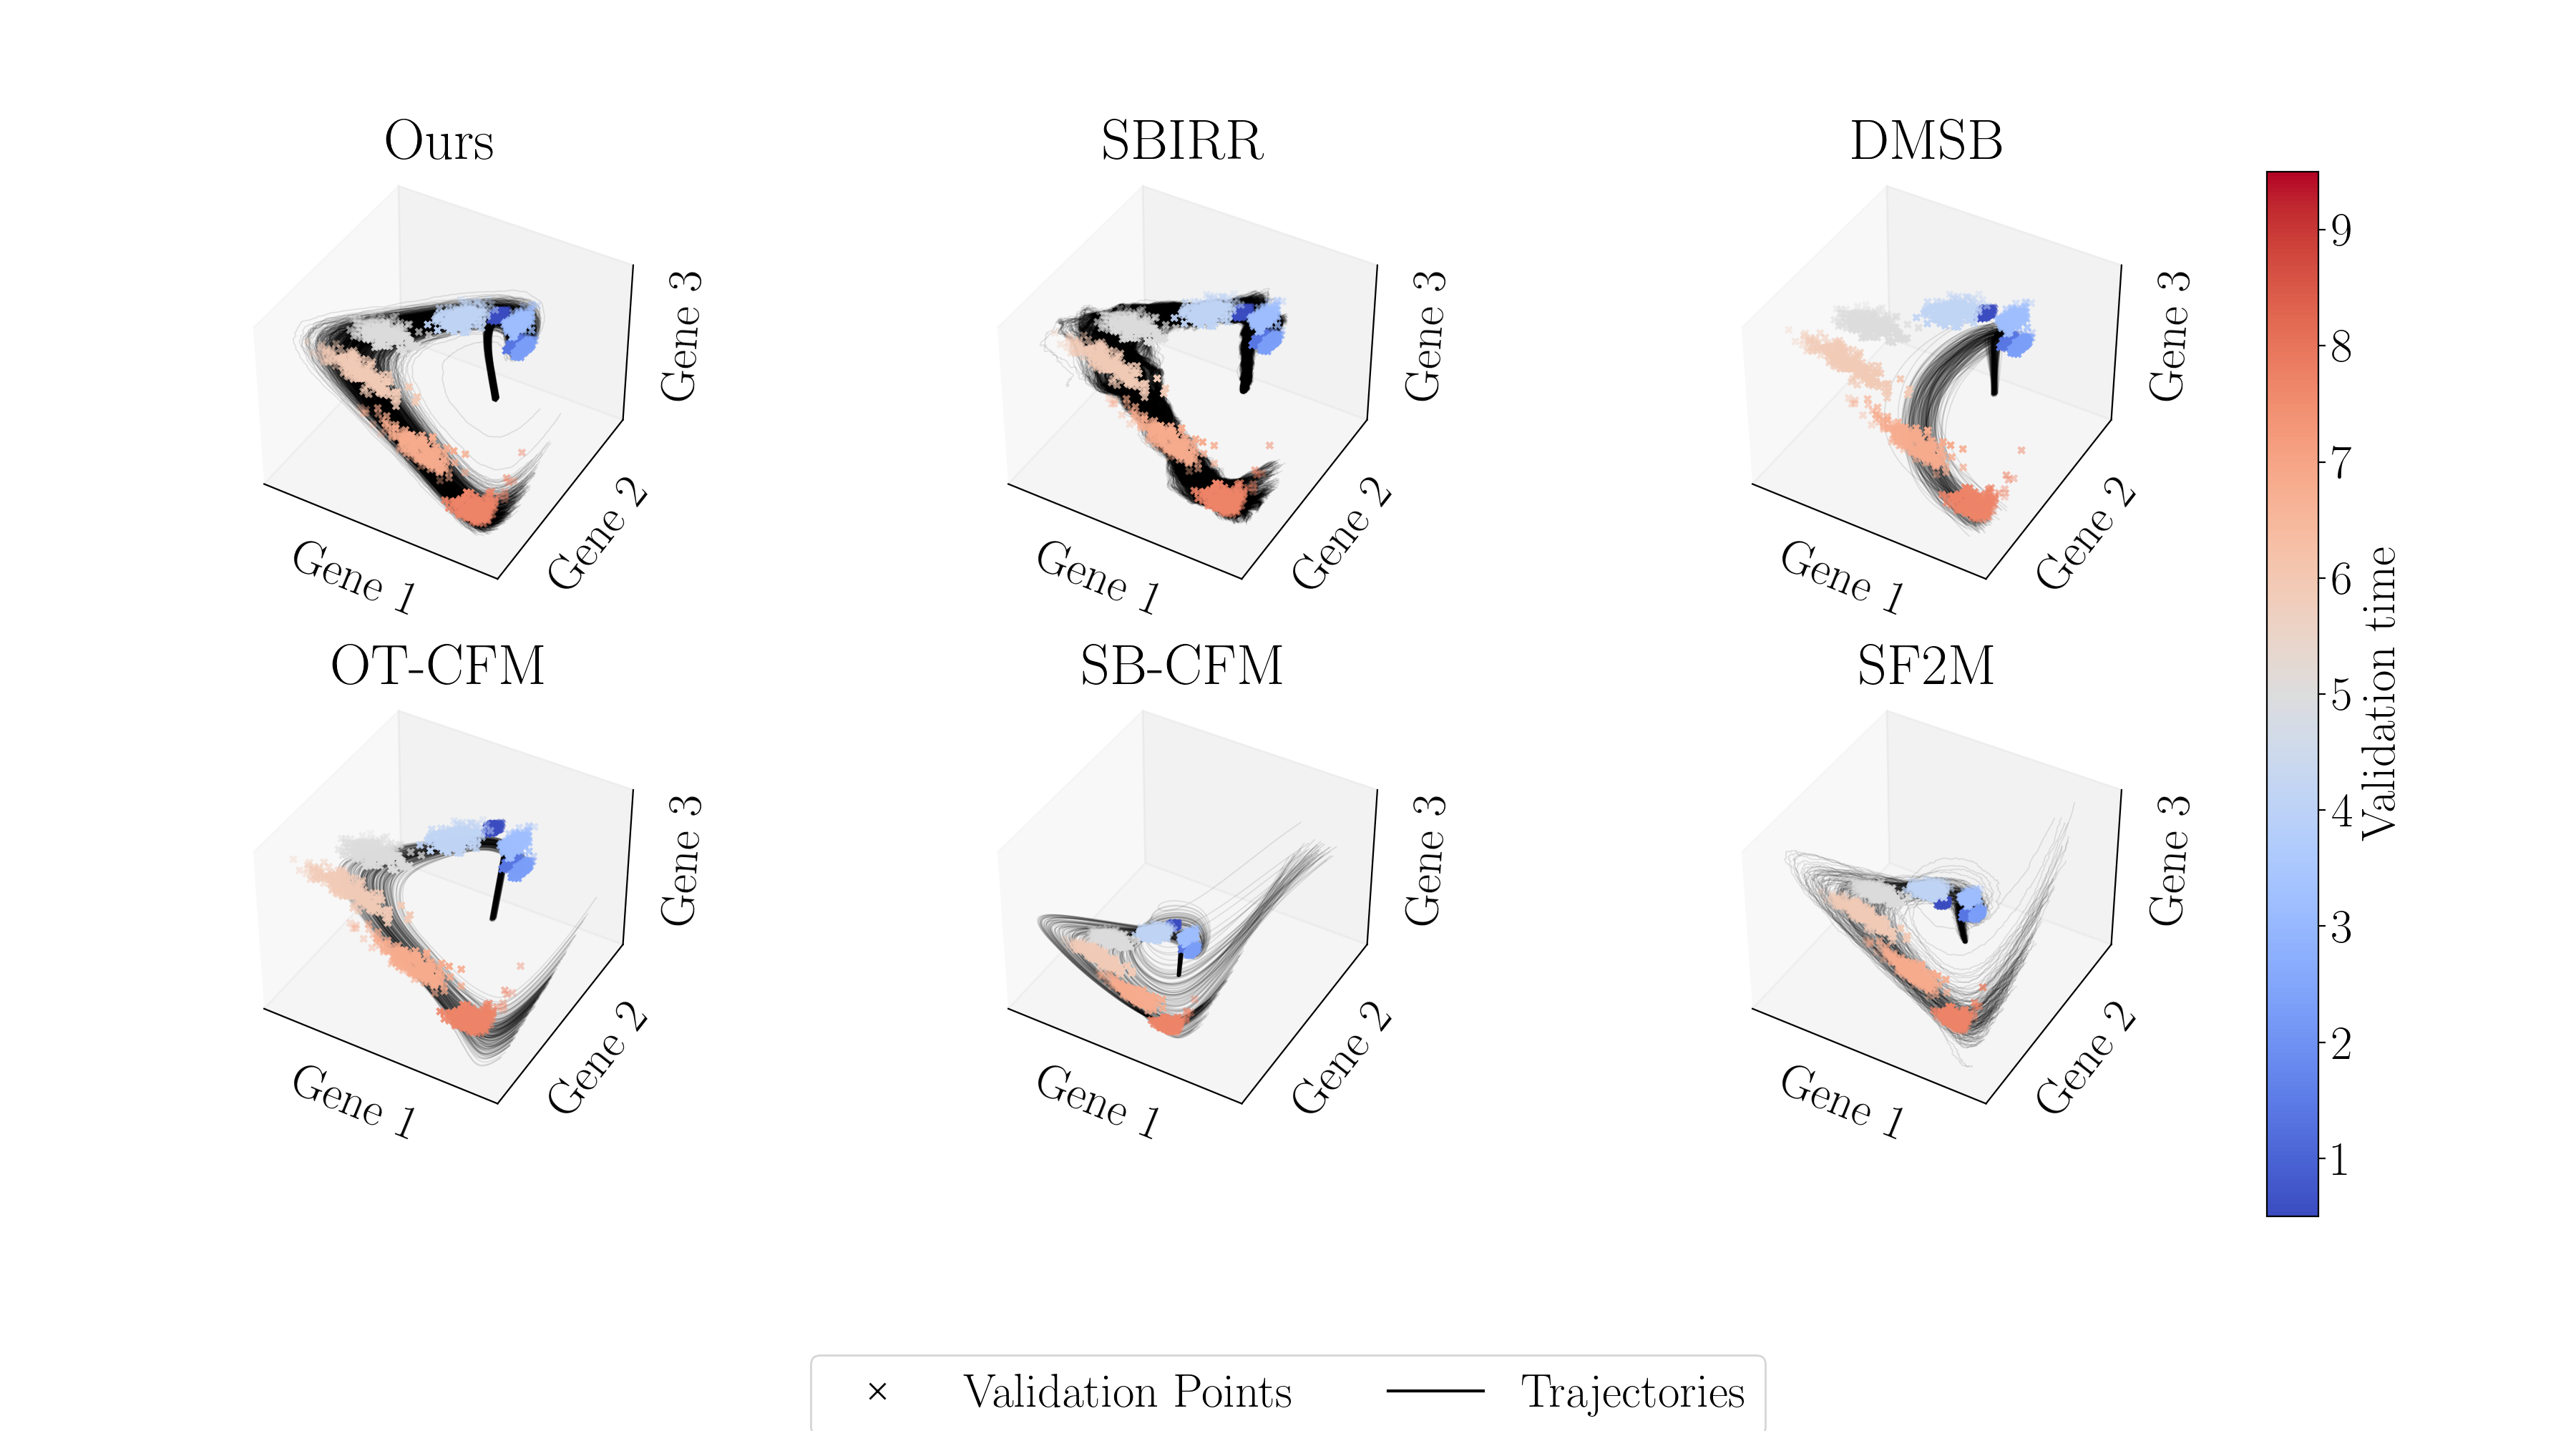
\includegraphics[width=\linewidth]{Figs/missingobs_Repressilator_interpolationing}

    \caption{Interpolation of repressilator system with missing protein.}
    \label{fig:repres-missing-protein-interpol}
\end{figure}

\begin{figure}[!ht]
    \centering
    \includegraphics[width=\linewidth]{Figs/Repressilator_missingobs_interpolation_metric.pdf}
    \caption{Metrics for Interpolation of repressilator system with missing protein.}
    \label{fig:repres-missing-protein-interpol-metric}
\end{figure}

\begin{table}[ht]
\caption{MMD at each validation point  for Repressilator with incomplete state observations.}
\centering
\makebox[0pt][c]{
\small
\begin{tabular}{lrrrrrr}
\toprule
Time & Ours & \texttt{SBIRR} & \texttt{DMSB} & \texttt{OT-CFM} & \texttt{SB-CFM} & \texttt{SF2M} \\\midrule
0.5 & \cellcolor{green!25}\bm{$0.015\pm{ 0.003}$} & $9.774\pm{ 0.027}$ & $9.847\pm{ 0.002}$ & $9.818\pm{ 0.010}$ & $9.745\pm{ 0.050}$ & $9.511\pm{ 0.121}$ \\
1.5 & \cellcolor{green!25}\bm{$0.019\pm{ 0.002}$} & $0.433\pm{ 0.357}$ & $3.606\pm{ 0.708}$ & $0.192\pm{ 0.158}$ & $0.531\pm{ 0.544}$ & $0.748\pm{ 0.688}$ \\
2.5 & \cellcolor{green!25}\bm{$0.004\pm{ 0.001}$} & $0.903\pm{ 0.131}$ & $2.990\pm{ 1.024}$ & $0.431\pm{ 0.129}$ & $0.688\pm{ 0.396}$ & $0.690\pm{ 0.306}$ \\
3.5 & \cellcolor{green!25}\bm{$0.009\pm{ 0.002}$} & $0.075\pm{ 0.032}$ & $3.642\pm{ 0.833}$ & $1.598\pm{ 0.789}$ & $1.578\pm{ 0.618}$ & $1.538\pm{ 0.503}$ \\
4.5 & \cellcolor{green!25}\bm{$0.008\pm{ 0.004}$} & $0.065\pm{ 0.026}$ & $6.131\pm{ 0.702}$ & $3.389\pm{ 1.494}$ & $2.254\pm{ 0.747}$ & $2.345\pm{ 0.764}$ \\
5.5 & \cellcolor{green!25}\bm{$0.010\pm{ 0.003}$} & $0.337\pm{ 0.038}$ & $8.024\pm{ 0.147}$ & $3.473\pm{ 0.950}$ & $2.431\pm{ 0.713}$ & $2.060\pm{ 0.470}$ \\
6.5 & \cellcolor{green!25}\bm{$0.014\pm{ 0.008}$} & $0.611\pm{ 0.112}$ & $7.033\pm{ 0.171}$ & $6.158\pm{ 0.735}$ & $2.953\pm{ 0.504}$ & $3.664\pm{ 0.506}$ \\
7.5 & \cellcolor{green!25}\bm{$0.007\pm{ 0.005}$} & $0.135\pm{ 0.053}$ & $2.830\pm{ 0.762}$ & $6.583\pm{ 0.499}$ & $2.850\pm{ 0.456}$ & $3.954\pm{ 0.553}$ \\
8.5 & \cellcolor{green!25}\bm{$0.011\pm{ 0.006}$} & $0.991\pm{ 0.191}$ & $2.223\pm{ 0.892}$ & $5.183\pm{ 0.978}$ & $2.869\pm{ 0.859}$ & $3.308\pm{ 0.446}$ \\
\bottomrule
\end{tabular}}
\label{tab:repr-missingobs-mmd}
\end{table}


\begin{table}[ht]
\caption{EMD at each validation point for Repressilator with incomplete state observations.}
\centering
\makebox[0pt][c]{
\small
\begin{tabular}{lrrrrrr}
\toprule
Time & Ours & \texttt{SBIRR} & \texttt{DMSB} & \texttt{OT-CFM} & \texttt{SB-CFM} & \texttt{SF2M} \\\midrule
0.5 & \cellcolor{green!25}\bm{$0.051\pm{ 0.003}$} & $2.721\pm{ 0.097}$ & $3.583\pm{ 0.071}$ & $2.596\pm{ 0.028}$ & $2.596\pm{ 0.029}$ & $2.578\pm{ 0.036}$ \\
1.5 & \cellcolor{green!25}\bm{$0.054\pm{ 0.002}$} & $0.209\pm{ 0.083}$ & $0.686\pm{ 0.086}$ & $0.166\pm{ 0.050}$ & $0.581\pm{ 0.675}$ & $0.874\pm{ 1.104}$ \\
2.5 & \cellcolor{green!25}\bm{$0.037\pm{ 0.001}$} & $0.317\pm{ 0.023}$ & $0.627\pm{ 0.131}$ & $0.225\pm{ 0.032}$ & $1.045\pm{ 2.139}$ & $1.823\pm{ 4.516}$ \\
3.5 & \cellcolor{green!25}\bm{$0.059\pm{ 0.002}$} & $0.120\pm{ 0.013}$ & $0.748\pm{ 0.111}$ & $0.449\pm{ 0.117}$ & $3.900\pm{ 9.557}$ & $7.221\pm{ 19.895}$ \\
4.5 & \cellcolor{green!25}\bm{$0.068\pm{ 0.004}$} & $0.144\pm{ 0.013}$ & $1.192\pm{ 0.145}$ & $0.794\pm{ 0.227}$ & $16.018\pm{ 44.580}$ & $30.671\pm{ 89.239}$ \\
5.5 & \cellcolor{green!25}\bm{$0.087\pm{ 0.005}$} & $0.246\pm{ 0.010}$ & $2.258\pm{ 0.192}$ & $0.826\pm{ 0.163}$ & $72.134\pm{ 212.668}$ & $136.803\pm{ 407.955}$ \\
6.5 & \cellcolor{green!25}\bm{$0.126\pm{ 0.011}$} & $0.437\pm{ 0.042}$ & $2.547\pm{ 0.200}$ & $2.346\pm{ 0.418}$ & $354.032\pm{ 1056.419}$ & $649.221\pm{ 1942.159}$ \\
7.5 & \cellcolor{green!25}\bm{$0.120\pm{ 0.006}$} & $0.324\pm{ 0.090}$ & $1.020\pm{ 0.136}$ & $2.614\pm{ 0.291}$ & $1691.087\pm{ 5066.068}$ & $2986.712\pm{ 8953.868}$ \\
8.5 & \cellcolor{green!25}\bm{$0.116\pm{ 0.005}$} & $0.802\pm{ 0.238}$ & $0.660\pm{ 0.150}$ & $1.934\pm{ 0.762}$ & $8102.608\pm{ 24292.997}$ & $13770.547\pm{ 41303.163}$ \\
\bottomrule
\end{tabular}}
\label{tab:repr-missingobs-emd}
\end{table}


\clearpage

\subsection{Current in the Gulf of Mexico}
\subsubsection{Experimental setup}
\label{app:gom-setup}
We test our method in fitting and forecasting real ocean-current data from the Gulf of Mexico. We use high-resolution (1 km) bathymetry data from a HYbrid Coordinate Ocean Model (HYCOM) reanalysis\footnote{Dataset available at \href{https://www.hycom.org/data/gomb0pt01/gom-reanalysis}{this link}.} \citep{panagiotis2014gulf}. This dataset has been in the public domain since it was released by the US Department of Defense. The dataset provides hourly ocean current velocity fields for the region extending from 98$^{\circ}$E to 77$^{\circ}$E in longitude and from 18$^{\circ}$N to 32$^{\circ}$N in latitude, covering every day since the first day of, 2001. 

We then generate particles following \citet{shen2024multi}. That is, we took the velocity field in a region where a vortex is observed in June 1st 2024 at 5pm. We then select an initial location near the vortex and uniformly sample 4,400 initial positions within a small radius ($0.05$) around this point and evolve these particles over 11 steps using the ocean current velocity field. The time step size is $1.0$ and left the last time step as validation. At each time point we retain 400 particles. We approximate the velocity at each particle's position using the velocity at the nearest grid point when the particle does not align exactly with a grid point. In addition, between each training time point, we simulate another 9 intermediate steps at middle point between each pair of consecutive training time points, with 400 particle each to test for interpolation. 

\subsubsection{Particle independence in the Gulf of Mexico experiment}
\label{app:gom_assumptions}
In the main text, we model particles at each time point as independent, without assuming continuity of individual trajectories across time. This reflects applications where repeated measurements of the same particle are not available. 

For example, if the particles were physical buoys or drifters deployed in the ocean, they could be tracked continuously, and trajectory-based methods would be more appropriate. By contrast, in many remote sensing applications each observation is an image that provides only a distributional snapshot at that time, without identifying or tracking the same particles across times. Oil-spill monitoring from satellite imagery is a common example: each image shows the surface oil distribution but not individual particle paths. Our Gulf of Mexico experiment is designed to mimic this setting and follows the procedure described in Appendix D.5.1 of \citet{shen2024multi}.


\subsubsection{Model family choice}
\label{app:gom_implementation}

We employ a physically motivated model to represent the vortex by combining a Lamb-Oseen vortex --- a solution of the two-dimensional viscous Navier-Stokes equations \citep{saffman1995vortex} --- with a constant divergence field. The Lamb-Oseen component captures the swirling, rotational dynamics typical of a vortex, while the divergence field is added to account for vertical motion or non-conservative forces that may cause a net expansion or contraction of the flow. In other words, this combined model enables us to represent both the core vortex behavior and the secondary effects influencing particle motion.

Formally, the particle trajectories are modeled by the following family of stochastic differential equations (SDEs):
\begin{equation}
    \begin{aligned}
        dX&=\left[-\gamma\frac{(Y-y_0)r_v}{(Y-y_0)^2+(Y-y_0)^2}\left(1-\exp\left(\frac{\sqrt{(Y-y_0)^2+(Y-y_0)^2}}{r_v}\right)\right)+d\frac{X-x_{0,d}}{r_d}  \right]dt+\sigma dW_x\\
        dY&=\left[\gamma\frac{(X-x_0)r_v}{(Y-y_0)^2+(Y-y_0)^2}\left(1-\exp\left(\frac{\sqrt{(Y-y_0)^2+(Y-y_0)^2}}{r_v}\right)\right)+d(Y-y_{0,d})  \right]dt+\sigma dW_y\\
    \end{aligned}
\end{equation}

In this formulation, the free parameters are:
\begin{itemize}
    \item Circulation ($\gamma$): Controls the strength of the vortex.
    \item Vortex length scale ($r_v$): Sets the radial decay of the vortex’s influence.
    \item Vortex center ($x_0, y_0$): Specifies the location of the vortex core.
    \item Divergence ($d$): Represents the magnitude of the constant divergence field.
    \item Divergence length scale ($r_d$): Governs the spatial extent of the divergence effect in the x-direction.
    \item Divergence center ($x_{0,d}, y_{0,d}$): Determines the reference location for the divergence field.
    \item Volatility ($\sigma$): Captures the stochastic fluctuations in particle motion.
\end{itemize}




\subsubsection{Forecasting results}
In this section, we further discuss results for the Gulf of Mexico vortex experiment. In particular, we analyze the EMD, MMD.

\begin{table}[!ht]
    \caption{Evaluation metric for Gulf of Mexico experiment (mean(sd)). Drift was evaluated using MSE on a grid.}
    \centering
    \begin{tabular}{lccc}
    \hline
    &     & Gulf of Mexico vortex & \\
    Metric     &  Ours & \texttt{SBIRR-ref} & \texttt{SB-forward} \\
    \hline
    Forecast-MMD & 2.36 (0.11) & \cellcolor{green!25}\textbf{1.41 (0.18)}& 2.59 (0.33) \\
    Forecast-EMD &  \cellcolor{green!25}\textbf{0.71(0.014)} & 0.89(0.034)& 0.94(0.081) \\
    Drift & 0.054 ($7.3\times 10^{-5}$) & \cellcolor{green!25}\textbf{0.031 (0.00032)} & 0.15 (0.023) \\
    \hline
    \end{tabular}

    \label{tab:GoM}
\end{table}

In the second row of \cref{tab:GoM}, we observe that our method achieves the lowest EMD for the forecasting task, indicating the closest match to the ground truth particle distribution. This aligns with the visual results in \cref{fig:GoMforecast} from the main text, where our forecasted particles accurately capture the spatial structure of the vortex, unlike the baselines which produce more scattered and less coherent predictions. While the MMD metric (first row) slightly favors the \texttt{SBIRR-ref} baseline, this discrepancy may be attributed to the sensitivity of MMD to particle density and kernel choice.

\subsubsection{Vector field reconstruction}
\label{app:gom-vector}
In the third row of \cref{tab:GoM}, we compare the drift reconstruction error using MSE on a grid. Here \texttt{SBIRR-ref} achieves the lowest error, and our method performs comparably and still significantly outperforms \texttt{SB-forward}. Visualizations in \cref{fig:gom-appendix} provide further insight: the reconstructed velocity fields from all the three methods exhibit a well-formed vortex structure closely resembling the ground truth (with our method and \texttt{SBIRR-ref} being slightly better, as also shown by the MSE results). 

\begin{figure}[!ht]
    \centering
    \includegraphics[width=\linewidth]{Figs/GoM_appendix_diff_arrows.pdf}
    \caption{Experimental results for the Gulf of Mexico experiment.}
    \label{fig:gom-appendix}
\end{figure}




\subsubsection{Interpolation}
\label{app:gom-interpol}

We now evaluate interpolation performance on the real-world drifter trajectories in the Gulf of Mexico. As shown in \cref{fig:GoM-interpol}, our method captures the overall geometry of the flow and the looping structure of the trajectories. All baselines also succeed in reconstructing the large-scale circulation, with \texttt{SBIRR} achieving the closest match to the held-out validation points. These patterns are reflected in the quantitative metrics in \cref{fig:GoM-interpol-metric} and tables \cref{tab:gom-mmd}–\cref{tab:gom-emd}: across nearly all validation times, \texttt{SBIRR} achieves the lowest MMD and EMD values, consistently outperforming our method and often the second-best method by a considerable margin.

This performance difference highlights a key distinction between modeling objectives. \texttt{SBIRR} is designed to directly interpolate between training marginals, and in this setting—where particles are relatively dense and the underlying flow field is smooth—interpolating training points naturally leads to trajectories that also pass near the validation points, which lie in between. In contrast, our method is not explicitly optimized to pass through the training marginals, but rather to estimate a smooth underlying velocity field from the available data. This distinction becomes particularly relevant in tasks such as forecasting, where the goal is to recover and extrapolate the underlying dynamics rather than simply interpolate known states.

\begin{figure}
    \centering
    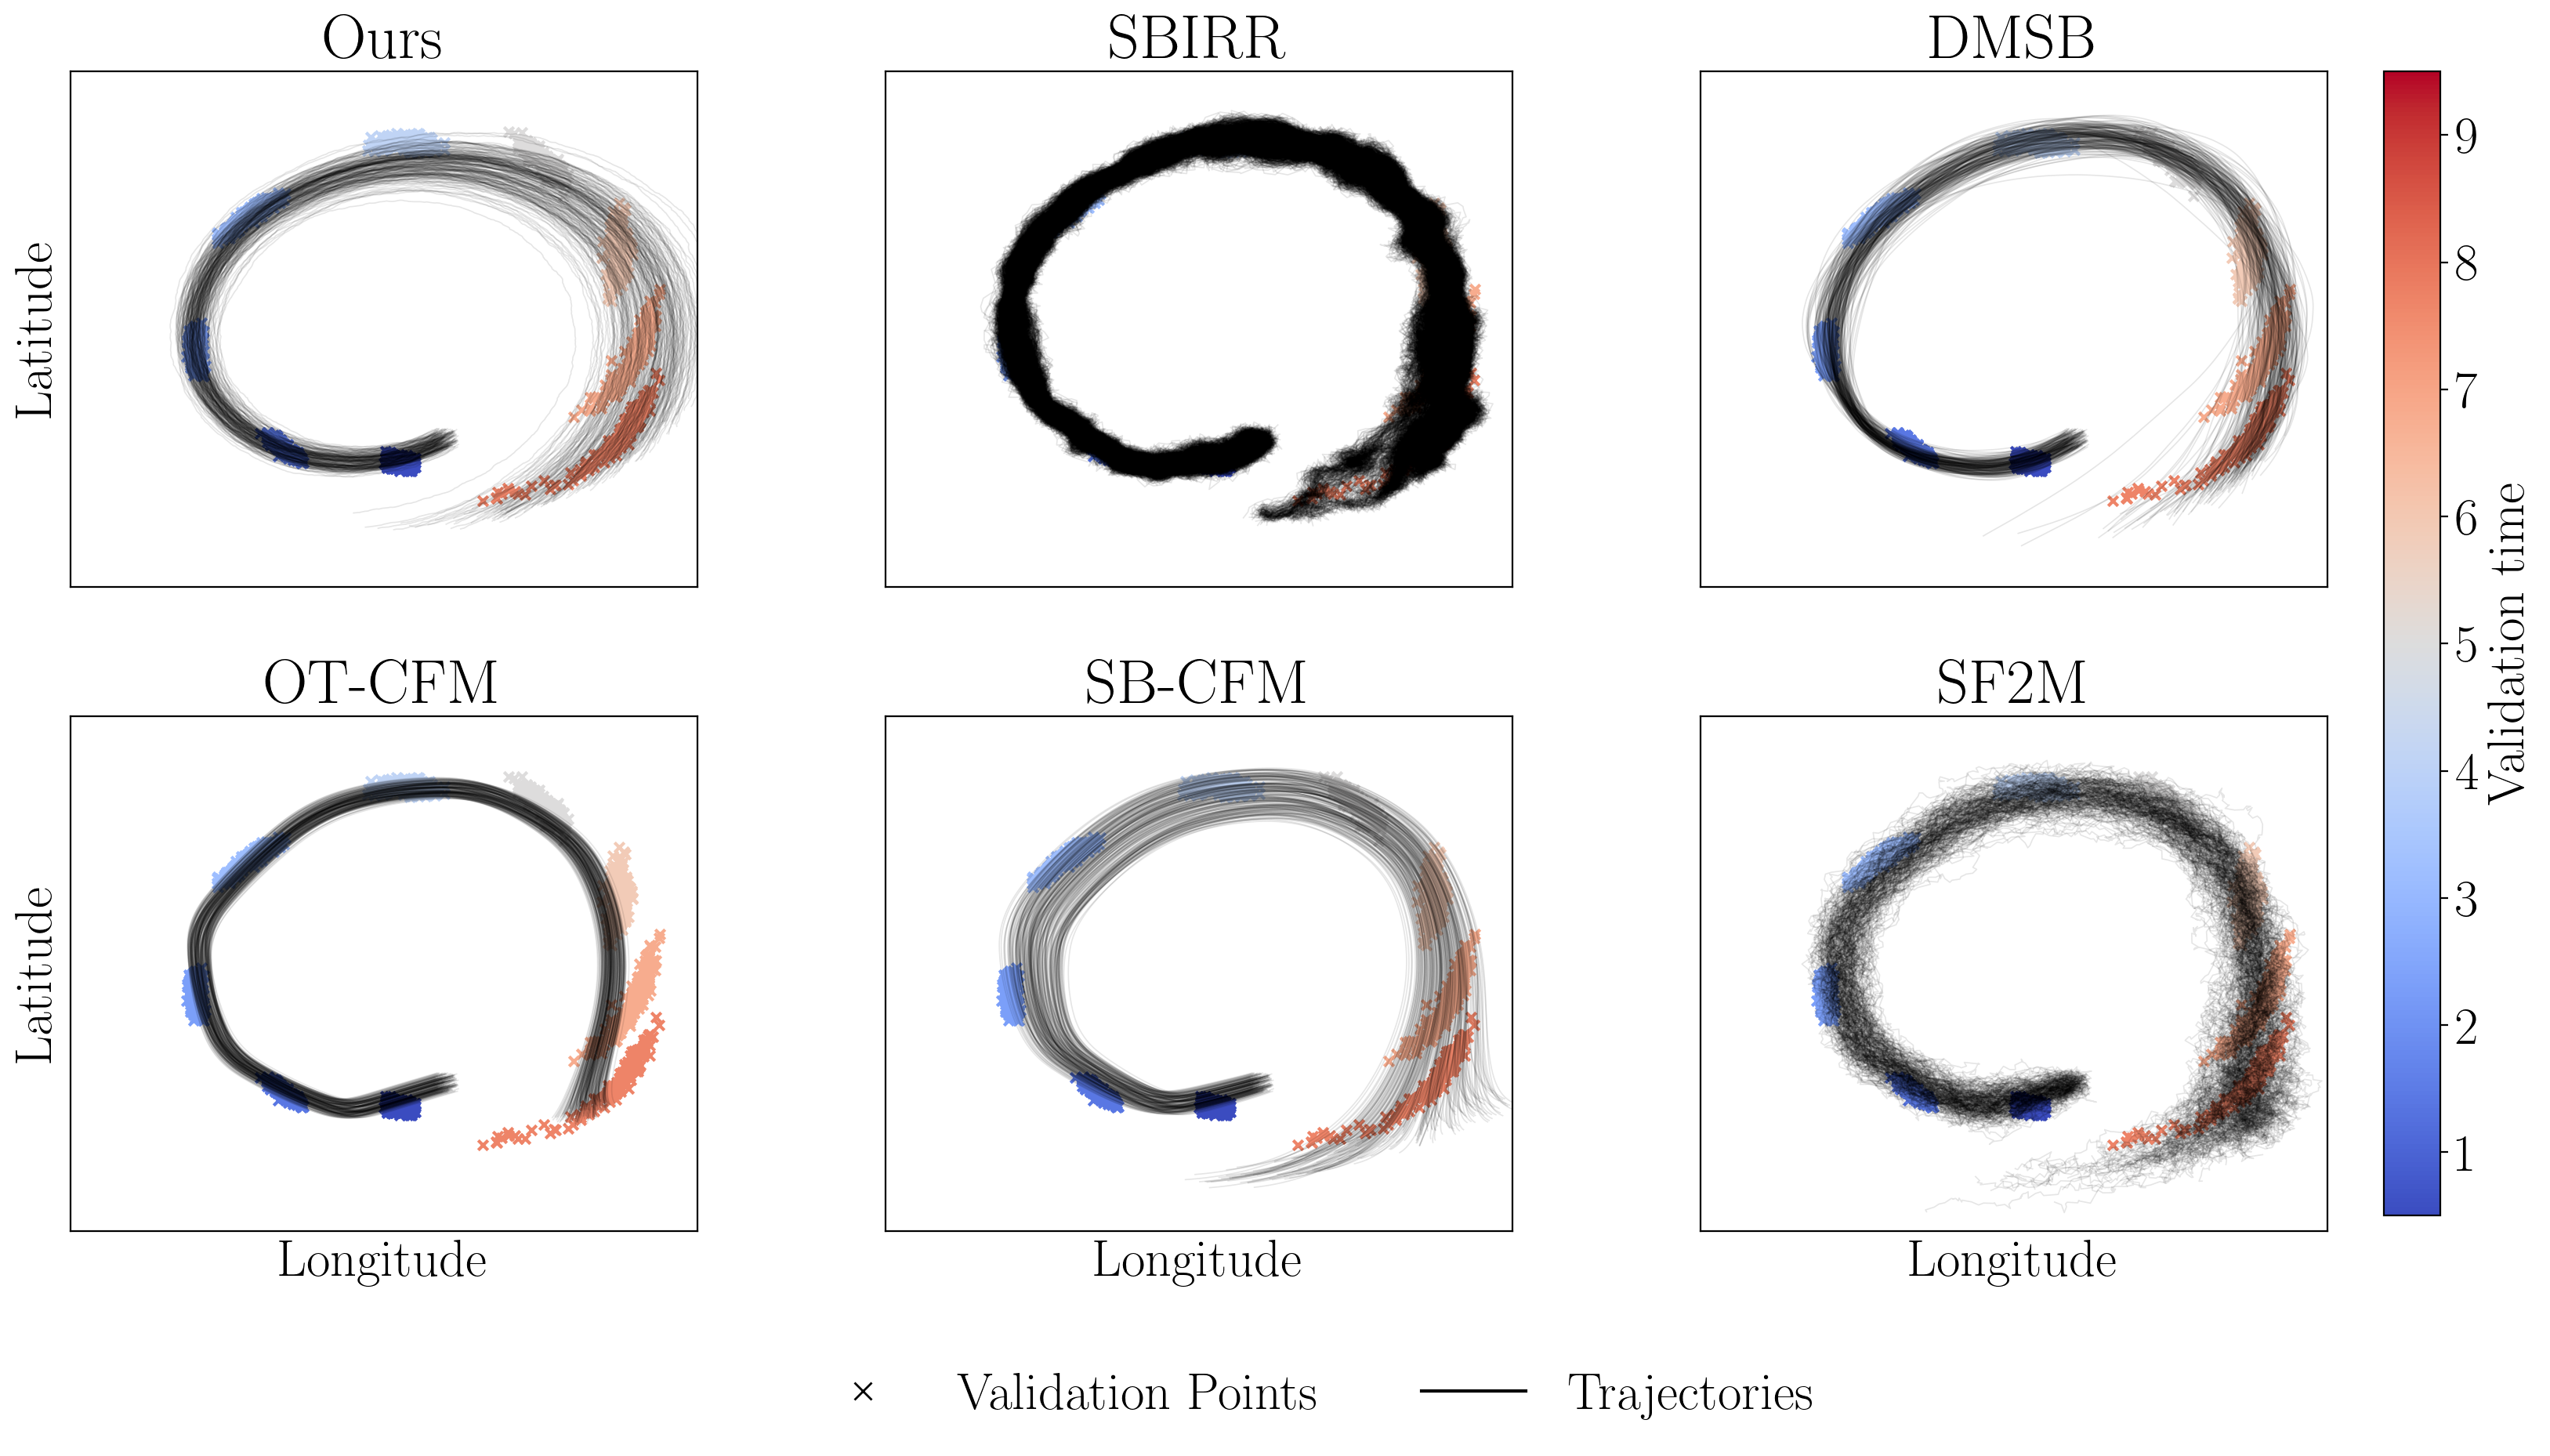
\includegraphics[width=\linewidth]{Figs/GoM_interpolationing.png}
    
    \caption{Interpolation of Gulf of Mexico current.}
    \label{fig:GoM-interpol}
\end{figure}

\begin{figure}
    \centering
    \includegraphics[width=\linewidth]{Figs/GoM_realdata_interpolation_metric.pdf}
    \caption{Metrics for Interpolation of Gulf of Mexico current.}
    \label{fig:GoM-interpol-metric}
\end{figure}

\begin{table}[ht]
\caption{MMD at each validation point for Gulf of Mexico.}
\centering
\makebox[0pt][c]{
\small
\begin{tabular}{lrrrrrr}
\toprule
Time & Ours & \texttt{SBIRR} & \texttt{DMSB} & \texttt{OT-CFM} & \texttt{SB-CFM} & \texttt{SF2M} \\\midrule
0.5 & $0.027\pm{ 0.001}$ & $0.011\pm{ 0.014}$ & \cellcolor{green!25}\bm{$0.005\pm{ 0.004}$} & $0.030\pm{ 0.002}$ & $0.030\pm{ 0.004}$ & $0.030\pm{ 0.004}$ \\
1.5 & $0.108\pm{ 0.004}$ & \cellcolor{green!25}\bm{$0.004\pm{ 0.004}$} & $0.030\pm{ 0.007}$ & $0.109\pm{ 0.013}$ & $0.097\pm{ 0.031}$ & $0.108\pm{ 0.013}$ \\
2.5 & $0.039\pm{ 0.003}$ & \cellcolor{green!25}\bm{$0.008\pm{ 0.006}$} & $0.021\pm{ 0.009}$ & $0.351\pm{ 0.043}$ & $0.353\pm{ 0.136}$ & $0.397\pm{ 0.030}$ \\
3.5 & $0.015\pm{ 0.002}$ & \cellcolor{green!25}\bm{$0.007\pm{ 0.007}$} & $0.064\pm{ 0.028}$ & $0.820\pm{ 0.123}$ & $0.854\pm{ 0.374}$ & $0.900\pm{ 0.090}$ \\
4.5 & $0.130\pm{ 0.007}$ & \cellcolor{green!25}\bm{$0.009\pm{ 0.005}$} & $0.031\pm{ 0.017}$ & $0.723\pm{ 0.160}$ & $0.797\pm{ 0.435}$ & $0.745\pm{ 0.093}$ \\
5.5 & $0.130\pm{ 0.010}$ & \cellcolor{green!25}\bm{$0.019\pm{ 0.009}$} & $0.036\pm{ 0.039}$ & $1.022\pm{ 0.205}$ & $1.049\pm{ 0.434}$ & $1.000\pm{ 0.070}$ \\
6.5 & $0.015\pm{ 0.005}$ & \cellcolor{green!25}\bm{$0.004\pm{ 0.005}$} & $0.114\pm{ 0.080}$ & $1.277\pm{ 0.248}$ & $1.192\pm{ 0.383}$ & $1.207\pm{ 0.139}$ \\
7.5 & $0.154\pm{ 0.023}$ & \cellcolor{green!25}\bm{$0.005\pm{ 0.003}$} & $0.133\pm{ 0.103}$ & $1.022\pm{ 0.271}$ & $1.000\pm{ 0.374}$ & $0.884\pm{ 0.192}$ \\
8.5 & $0.037\pm{ 0.006}$ & \cellcolor{green!25}\bm{$0.005\pm{ 0.007}$} & $0.040\pm{ 0.044}$ & $0.507\pm{ 0.239}$ & $0.867\pm{ 0.772}$ & $0.348\pm{ 0.141}$ \\
\bottomrule
\end{tabular}}
\label{tab:gom-mmd}
\end{table}


\begin{table}[ht]
\caption{EMD at each validation point for Gulf of Mexico.}
\centering
\makebox[0pt][c]{
\small
\begin{tabular}{lrrrrrr}
\toprule
Time & Ours & \texttt{SBIRR} & \texttt{DMSB} & \texttt{OT-CFM} & \texttt{SB-CFM} & \texttt{SF2M} \\\midrule
0.5 & $0.054\pm{ 0.001}$ & $0.041\pm{ 0.017}$ & \cellcolor{green!25}\bm{$0.025\pm{ 0.007}$} & $0.057\pm{ 0.002}$ & $0.057\pm{ 0.004}$ & $0.068\pm{ 0.004}$ \\
1.5 & $0.109\pm{ 0.002}$ & \cellcolor{green!25}\bm{$0.033\pm{ 0.007}$} & $0.058\pm{ 0.007}$ & $0.109\pm{ 0.006}$ & $0.104\pm{ 0.015}$ & $0.114\pm{ 0.007}$ \\
2.5 & $0.072\pm{ 0.002}$ & \cellcolor{green!25}\bm{$0.038\pm{ 0.009}$} & $0.054\pm{ 0.009}$ & $0.194\pm{ 0.012}$ & $0.194\pm{ 0.037}$ & $0.210\pm{ 0.009}$ \\
3.5 & $0.055\pm{ 0.002}$ & \cellcolor{green!25}\bm{$0.039\pm{ 0.011}$} & $0.092\pm{ 0.017}$ & $0.301\pm{ 0.024}$ & $0.303\pm{ 0.069}$ & $0.318\pm{ 0.016}$ \\
4.5 & $0.122\pm{ 0.003}$ & \cellcolor{green!25}\bm{$0.041\pm{ 0.010}$} & $0.079\pm{ 0.013}$ & $0.277\pm{ 0.033}$ & $0.289\pm{ 0.081}$ & $0.286\pm{ 0.017}$ \\
5.5 & $0.126\pm{ 0.004}$ & \cellcolor{green!25}\bm{$0.055\pm{ 0.009}$} & $0.070\pm{ 0.023}$ & $0.333\pm{ 0.036}$ & $0.342\pm{ 0.073}$ & $0.336\pm{ 0.012}$ \\
6.5 & $0.071\pm{ 0.005}$ & \cellcolor{green!25}\bm{$0.037\pm{ 0.007}$} & $0.109\pm{ 0.036}$ & $0.379\pm{ 0.040}$ & $0.374\pm{ 0.062}$ & $0.374\pm{ 0.023}$ \\
7.5 & $0.158\pm{ 0.009}$ & \cellcolor{green!25}\bm{$0.048\pm{ 0.009}$} & $0.121\pm{ 0.043}$ & $0.351\pm{ 0.046}$ & $0.358\pm{ 0.071}$ & $0.324\pm{ 0.038}$ \\
8.5 & $0.160\pm{ 0.008}$ & \cellcolor{green!25}\bm{$0.053\pm{ 0.011}$} & $0.094\pm{ 0.029}$ & $0.264\pm{ 0.049}$ & $0.361\pm{ 0.163}$ & $0.210\pm{ 0.045}$ \\
\bottomrule
\end{tabular}}
\label{tab:gom-emd}
\end{table}


\clearpage



\subsection{T cell-mediated immune activation}
In this section, we describe details of the T cell-mediated immune activation experiment contained in the main text. The dataset was released with the paper by \citet{jiang2024d} under CC-BY-NC 4.0 international license. 
\subsubsection{Background for the biological experiment.}
\label{app:pbmc-biology}
\paragraph{Peripheral blood mononuclear cells}
Peripheral blood mononuclear cells (PBMCs) comprise a heterogeneous mixture of immune cells, including T cells, B cells, natural killer (NK) cells, and myeloid lineages.  
To trigger a coordinated immune response, the PBMC pool from a single healthy donor was stimulated \emph{in vitro} with anti-CD3/CD28 antibodies at $t=0$ to selectively induce T cell activation.   
Cytokines released by activated T cells subsequently induce transcriptional changes and subsequent cytokine communications in the immune cell populations, yielding a rich, system-wide dynamical process.

\paragraph{Data acquisition.}
Cells were sampled every 30 min for 30 h (61 time points) and profiled with multiplexed single-cell mRNA sequencing \citep{jiang2024d}.  Raw counts were library-size normalised and log-transformed following standard scRNA-seq workflows.  
Each snapshot is very high-dimensional (there are hundreds of cells and thousands of genes for each cell). 
Because modelling all genes directly is infeasible and biologically redundant, we adopt the widely used \emph{gene-program} formulation: groups of co-expressed genes are collapsed into latent variables that capture coordinated transcriptional activity.  

\subsubsection{Experiment setup}
\label{app:pbmc-setup}
We use the 30 biologically annotated programs in \citet{jiang2024d} together with the dataset, which was computed from orthogonal non-negative matrix factorisation (oNMF) \citep{ding2006orthogonal}. Projecting each cell onto this 30-dimensional program space yields a low-noise, interpretable representation that is well suited for dynamical modelling. We took data from 0-20 hours (41 snapshots in total), before the cells reached steady state. We train our model using data at $0, 1, \dots, 19$th hours for training, left measurement at $20$th hour to test for forecast, and left $0.5, 1.5, \dots, 18.5$th hour to test for interpolation. We show in \cref{fig:pbmc-training-progression} the evolution of the 20 training points and the forecast validation time point (bottom-left).

\begin{figure}
    \centering
    \includegraphics[width=.85\linewidth]{Figs/pbmc_forecasting_progression_6x4.pdf}
    \caption{Training data for the PBMC experiment and forecasts with the three methods.}
    \label{fig:pbmc-training-progression}
\end{figure}

\subsubsection{Model family choice}
\label{app:pbmc-implementation}
We employ the architecture of \cref{eq:mlpactive}, instantiated with a 30-dimensional state space.  
The drift is parameterised by a three-layer MLP with hidden widths $[128,128,128]$, ReLU activations and a sigmoid output that keeps gene-program values within biologically plausible bounds.  
Hyper-parameters were chosen via a small grid search (two vs. three layers, and 32 vs. 64 vs. 128 hidden nodes per layer) on the $R^{2}$ score.

\subsubsection{Forecasting results}
\label{app:pbmc-forecast}
Table~\ref{tab:repr-pbmc} reports quantitative forecasting performance.  
Because the ground-truth vector field is unknown, we restrict evaluation to distributional metrics.  
EMD solver failed to converge in 30 dimensions, so we use MMD with an RBF kernel of bandwidth~1.  
Our method attains an MMD that is an order of magnitude lower than either baseline, confirming the qualitative superiority observed in \cref{fig:pbmc-forecasting}.  

\begin{table}[!ht]
    \centering
    \caption{One-step-ahead forecasting error on the T-cell activation dataset (mean $\pm$ s.d.\ over 10 seeds). MMD is computed with an RBF kernel of bandwidth 1 after scaling each gene program to unit variance. EMD is not reported because the solver failed to converge in 30 dimensions.}
    \begin{tabular}{lccc}
    \hline
    &     & pbmc & \\
    Metric     &  Ours & \texttt{SBIRR-ref} & \texttt{SB-forward} \\
    \hline
    Forecast-MMD & \cellcolor{green!25}\textbf{0.11 (0.04)} & 0.69 (0.11)& 2.99 (1.88) \\
    \hline
    \end{tabular}

    \label{tab:repr-pbmc}
\end{table}

\subsubsection{Interpolation}
\label{app:pbmc-interpol}

We now assess interpolation performance on this real-world single-cell dataset. As shown in \cref{fig:pbmc-interpol}, our method produces biologically plausible trajectories that span the principal components of the data and remain well-aligned with the progression of held-out validation points. \texttt{SBIRR}, \texttt{OT-CFM} , and \texttt{SB-CFM}  perform similarly well in this task, whereas \texttt{DMSB}  produces notably erratic paths with high variance, and \texttt{SF2M}  displays more diffuse interpolations. The same pattern appears if we look at interpolation predictions across the validation time steps, as shown in \cref{fig:pbmc-interpolation-1-5}, \cref{fig:pbmc-interpolation-6-10}, \cref{fig:pbmc-interpolation-11-15}, and \cref{fig:pbmc-interpolation-16-20}. In particular, we see that our method and \texttt{SBIRR} produce quite accurate interpolations for most of the time steps. Quantitative results in \cref{fig:pbmc-interpol-metric} and \cref{tab:pbmc-mmd} support these impressions. Across the full time course, our method consistently achieves the lowest MMD at most validation points, often by a statistically significant margin. \texttt{SBIRR} performs competitively, particularly at later times, while the performance of \texttt{DMSB}  degrades substantially, as reflected by persistently high MMD values throughout the trajectory. We note that, in contrast to previous experiments, we do not report EMD in this setting. Due to the high dimensionality of the latent space (30 dimensions), EMD becomes increasingly unreliable as a metric, suffering from the curse of dimensionality and producing unstable estimates. For this reason, we focus our evaluation on MMD, which remains well-behaved in high-dimensional settings and provides a more robust comparison of distributional fidelity across methods.

\begin{figure}[!ht]
    \centering
    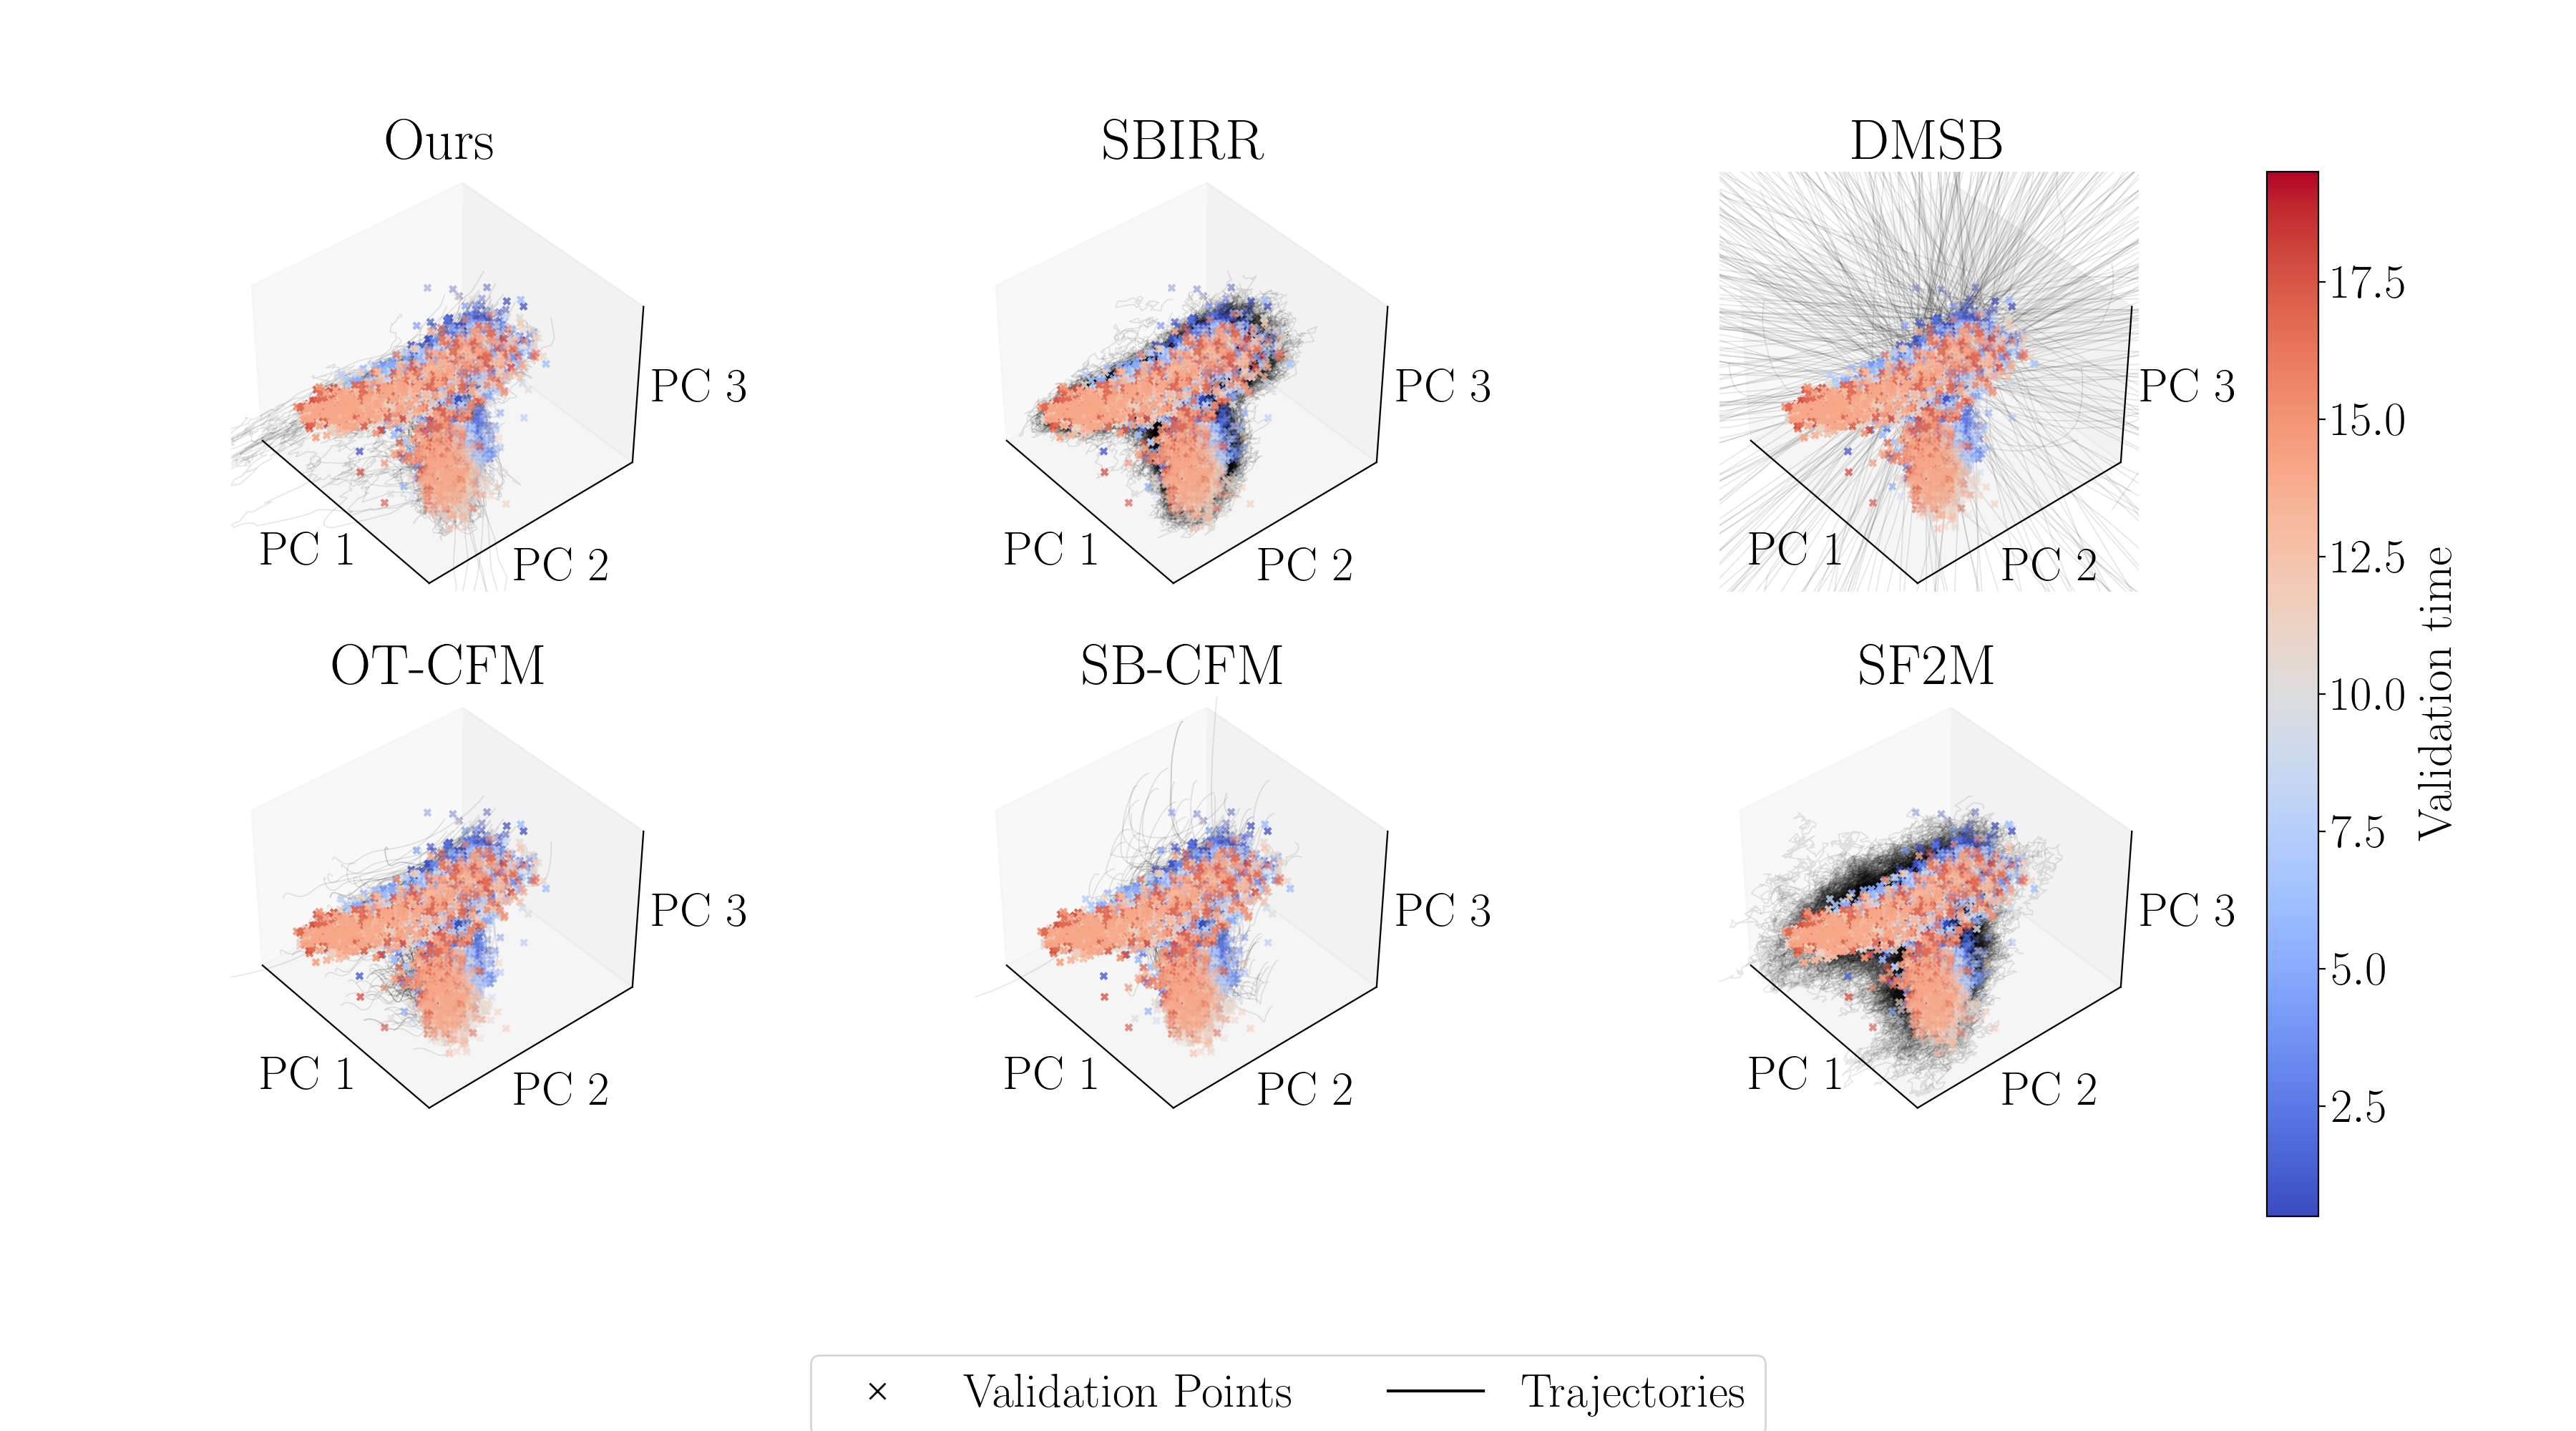
\includegraphics[width=\linewidth]{Figs/pbmc_interpolationing.png}
    
    \caption{Interpolation of pbmc dataset. }
    \label{fig:pbmc-interpol}
\end{figure}

\begin{figure}[!ht]
    \centering
    \includegraphics[width=.85\linewidth]{Figs/pbmc_interpolation_grid_1.pdf}
    \caption{PBMC interpolation results for the first 5 validation time points. The axis are the first three principal components as in the forecasting experiment. The first row shows the evolution of cells for ground truth. The other six rows show the predicted cells at the validation time points for the our method and the five baselines.}
    \label{fig:pbmc-interpolation-1-5}
\end{figure}

\begin{figure}[!ht]
    \centering
    \includegraphics[width=.85\linewidth]{Figs/pbmc_interpolation_grid_2.pdf}
    \caption{PBMC interpolation results for validation time points 6 to 10. The axis are the first three principal components as in the forecasting experiment. The first row shows the evolution of cells for ground truth. The other six rows show the predicted cells at the validation time points for the our method and the five baselines.}
    \label{fig:pbmc-interpolation-6-10}
\end{figure}

\begin{figure}[!ht]
    \centering
    \includegraphics[width=.85\linewidth]{Figs/pbmc_interpolation_grid_3.pdf}
    \caption{PBMC interpolation results for validation time points 11 to 15. The axis are the first three principal components as in the forecasting experiment. The first row shows the evolution of cells for ground truth. The other six rows show the predicted cells at the validation time points for the our method and the five baselines.}
    \label{fig:pbmc-interpolation-11-15}
\end{figure}

\begin{figure}[!ht]
    \centering
    \includegraphics[width=.85\linewidth]{Figs/pbmc_interpolation_grid_4.pdf}
    \caption{PBMC interpolation results for validation time points 16 to 20. The axis are the first three principal components as in the forecasting experiment. The first row shows the evolution of cells for ground truth. The other six rows show the predicted cells at the validation time points for the our method and the five baselines.}
    \label{fig:pbmc-interpolation-16-20}
\end{figure}

\begin{figure}[!ht]
    \centering
    \includegraphics[width=\linewidth]{Figs/pbmc_realdata_interpolation_metric.pdf}
    \caption{Metrics for Interpolation of pbmc dataset. }
    \label{fig:pbmc-interpol-metric}
\end{figure}

\begin{table}[ht]
\caption{MMD at each validation point for PBMC.}
\centering
\makebox[0pt][c]{
\small
\begin{tabular}{lrrrrrr}
\toprule
Time & Ours & \texttt{SBIRR} & \texttt{DMSB} & \texttt{OT-CFM} & \texttt{SB-CFM} & \texttt{SF2M} \\\midrule
0.5 & \cellcolor{green!25}$0.310\pm{ 0.013}$ & $0.610\pm{ 0.052}$ & $0.853\pm{ 0.041}$ & $0.318\pm{ 0.010}$ & $0.328\pm{ 0.009}$ & \cellcolor{green!25}\bm{$0.306\pm{ 0.008}$} \\
1.5 & \cellcolor{green!25}\bm{$0.125\pm{ 0.010}$} & $0.189\pm{ 0.022}$ & $0.803\pm{ 0.001}$ & $0.183\pm{ 0.029}$ & $0.201\pm{ 0.018}$ & $0.163\pm{ 0.019}$ \\
2.5 & \cellcolor{green!25}\bm{$0.125\pm{ 0.011}$} & $0.175\pm{ 0.012}$ & $0.804\pm{ 0.000}$ & $0.264\pm{ 0.053}$ & $0.270\pm{ 0.053}$ & $0.236\pm{ 0.050}$ \\
3.5 & \cellcolor{green!25}\bm{$0.126\pm{ 0.012}$} & $0.148\pm{ 0.015}$ & $0.839\pm{ 0.000}$ & $0.309\pm{ 0.064}$ & $0.308\pm{ 0.059}$ & $0.265\pm{ 0.050}$ \\
4.5 & $0.132\pm{ 0.019}$ & \cellcolor{green!25}\bm{$0.060\pm{ 0.009}$} & $0.898\pm{ 0.000}$ & $0.275\pm{ 0.069}$ & $0.294\pm{ 0.059}$ & $0.258\pm{ 0.051}$ \\
5.5 & $0.144\pm{ 0.016}$ & \cellcolor{green!25}\bm{$0.092\pm{ 0.010}$} & $1.019\pm{ 0.000}$ & $0.318\pm{ 0.081}$ & $0.339\pm{ 0.063}$ & $0.301\pm{ 0.049}$ \\
6.5 & $0.106\pm{ 0.013}$ & \cellcolor{green!25}\bm{$0.061\pm{ 0.007}$} & $0.939\pm{ 0.000}$ & $0.335\pm{ 0.096}$ & $0.357\pm{ 0.072}$ & $0.295\pm{ 0.049}$ \\
7.5 & $0.081\pm{ 0.009}$ & \cellcolor{green!25}\bm{$0.030\pm{ 0.005}$} & $0.948\pm{ 0.000}$ & $0.342\pm{ 0.107}$ & $0.375\pm{ 0.087}$ & $0.292\pm{ 0.056}$ \\
8.5 & $0.093\pm{ 0.011}$ & \cellcolor{green!25}\bm{$0.037\pm{ 0.003}$} & $1.052\pm{ 0.000}$ & $0.374\pm{ 0.122}$ & $0.422\pm{ 0.097}$ & $0.329\pm{ 0.054}$ \\
9.5 & $0.100\pm{ 0.016}$ & \cellcolor{green!25}\bm{$0.039\pm{ 0.002}$} & $1.081\pm{ 0.000}$ & $0.396\pm{ 0.130}$ & $0.456\pm{ 0.105}$ & $0.353\pm{ 0.056}$ \\
10.5 & \cellcolor{green!25}\bm{$0.118\pm{ 0.018}$} & \cellcolor{green!25}$0.122\pm{ 0.010}$ & $1.092\pm{ 0.000}$ & $0.528\pm{ 0.150}$ & $0.569\pm{ 0.126}$ & $0.425\pm{ 0.068}$ \\
11.5 & $0.077\pm{ 0.010}$ & \cellcolor{green!25}\bm{$0.069\pm{ 0.007}$} & $1.066\pm{ 0.000}$ & $0.505\pm{ 0.154}$ & $0.554\pm{ 0.131}$ & $0.397\pm{ 0.074}$ \\
12.5 & $0.073\pm{ 0.010}$ & \cellcolor{green!25}\bm{$0.059\pm{ 0.006}$} & $1.023\pm{ 0.000}$ & $0.519\pm{ 0.156}$ & $0.567\pm{ 0.129}$ & $0.388\pm{ 0.073}$ \\
13.5 & $0.093\pm{ 0.014}$ & \cellcolor{green!25}\bm{$0.066\pm{ 0.004}$} & $1.004\pm{ 0.000}$ & $0.573\pm{ 0.163}$ & $0.621\pm{ 0.130}$ & $0.417\pm{ 0.070}$ \\
14.5 & $0.096\pm{ 0.016}$ & \cellcolor{green!25}\bm{$0.071\pm{ 0.010}$} & $1.131\pm{ 0.000}$ & $0.591\pm{ 0.196}$ & $0.679\pm{ 0.151}$ & $0.448\pm{ 0.080}$ \\
15.5 & $0.101\pm{ 0.016}$ & \cellcolor{green!25}\bm{$0.085\pm{ 0.008}$} & $0.942\pm{ 0.000}$ & $0.533\pm{ 0.163}$ & $0.601\pm{ 0.125}$ & $0.360\pm{ 0.058}$ \\
16.5 & \cellcolor{green!25}$0.111\pm{ 0.015}$ & \cellcolor{green!25}\bm{$0.108\pm{ 0.017}$} & $1.019\pm{ 0.000}$ & $0.594\pm{ 0.183}$ & $0.683\pm{ 0.130}$ & $0.414\pm{ 0.060}$ \\
17.5 & \cellcolor{green!25}$0.077\pm{ 0.019}$ & \cellcolor{green!25}\bm{$0.071\pm{ 0.015}$} & $0.978\pm{ 0.000}$ & $0.598\pm{ 0.190}$ & $0.688\pm{ 0.141}$ & $0.404\pm{ 0.060}$ \\
18.5 & \cellcolor{green!25}$0.089\pm{ 0.023}$ & \cellcolor{green!25}\bm{$0.089\pm{ 0.015}$} & $0.896\pm{ 0.000}$ & $0.616\pm{ 0.185}$ & $0.698\pm{ 0.134}$ & $0.385\pm{ 0.055}$ \\
19.5 & \cellcolor{green!25}\bm{$0.099\pm{ 0.034}$} & \cellcolor{green!25}$0.107\pm{ 0.022}$ & $0.971\pm{ 0.000}$ & $0.637\pm{ 0.204}$ & $0.753\pm{ 0.146}$ & $0.425\pm{ 0.063}$ \\
\bottomrule
\end{tabular}}
\label{tab:pbmc-mmd}
\end{table}




\clearpage

\section{Ablation Studies Full Results}
\label{app:ablations}

In this appendix, we present extended results for the ablation studies from Section~\ref{sec:ablations}. 
We consider two settings: (i) replacing learned, state-dependent volatility with a fixed scalar volatility, and (ii) replacing structured SDE drift/volatility with a fully neural parameterization. 
Tables report mean, standard deviation, and range across seeds for both SnapMMD and the ablated variants.


\subsection{Impact of learning state-dependent volatility}
\label{app:ablation-fixed}

In our main experiments, SnapMMD learns a volatility term that may vary with state. 
Here we ablate this feature by fixing volatility to a constant scalar across states and times (set to $0.1$ following prior SB work). 

Across tasks, learning volatility yields clear benefits: 
in Lotka--Volterra and parametric Repressilator, MMD errors fall by more than an order of magnitude relative to fixed volatility, reflecting the importance of capturing heterogeneous noise levels. 
In PBMC, the fixed-volatility variant shows large instability across seeds (variance over an order of magnitude), while learned volatility produces consistently low error. 
The only exception is the Gulf of Mexico forecasting task, where fixed volatility yields more diffuse predictions that happen to align better with the kernel geometry used in the MMD metric. 
Importantly, even in this case, SnapMMD with learned volatility performs better on the interpolation task, where the goal is reconstructing observed marginals rather than extrapolating. 




\begin{table}[ht]
\centering
\caption{Forecasting performance: SnapMMD with learned state-dependent diffusion vs.\ fixed diffusion.}
\label{tab:abl-fixed-forecast}
\begin{tabular}{lcccccc}
\toprule
& \multicolumn{3}{c}{SnapMMD (learned volatility)} & \multicolumn{3}{c}{Fixed volatility} \\
\cmidrule(lr){2-4} \cmidrule(lr){5-7}
Experiment & Mean & SD & Range & Mean & SD & Range \\
\midrule
LV            & 0.057 & 0.030 & [0.025, 0.122] & 0.156 & 0.020 & [0.128, 0.189] \\
ReprParam     & 0.072 & 0.080 & [0.005, 0.243] & 7.557 & 0.001 & [7.555, 7.559] \\
ReprSemiparam & 0.320 & 0.150 & [0.150, 0.640] & 0.286 & 0.191 & [0.035, 0.656] \\
ReprProtein& 0.067 & 0.034 & [0.018, 0.116] & 0.072   & 0.023   & [0.041, 0.128]   \\
GoM           & 2.360 & 0.110 & [2.192, 2.582] & 0.969 & 0.398 & [0.654, 2.079] \\
PBMC          & 0.110 & 0.040 & [0.077, 0.236] & 0.376 & 0.542 & [0.077, 1.667] \\
\bottomrule
\end{tabular}
\end{table}



\begin{table}[ht]
\centering
\caption{Interpolation performance: SnapMMD with learned state-dependent diffusion vs.\ fixed volatility. 
We report mean, standard deviation, and range across seeds.}
\label{tab:abl-fixed-interp}
\begin{tabular}{lcccccc}
\toprule
& \multicolumn{3}{c}{SnapMMD (learned volatility)} & \multicolumn{3}{c}{Fixed volatility} \\
\cmidrule(lr){2-4} \cmidrule(lr){5-7}
Experiment & Mean & SD & Range & Mean & SD & Range \\
\midrule
LV & 0.013 & 0.011 & [0.000, 0.075] & 8.771 & 2.257 & [1.599, 9.917] \\
ReprParam & 0.040 & 0.034 & [0.002, 0.166] & 8.461 & 0.588 & [7.693, 9.570] \\
ReprSemiparam & 0.379 & 0.381 & [0.005, 1.459] & 8.423 & 1.770 & [2.643, 9.919] \\
ReprProtein & 0.011 & 0.006 & [0.002, 0.034] & 8.768 & 1.350 & [4.074, 9.889] \\
GoM & 0.073 & 0.054 & [0.007, 0.200] & 6.716 & 3.156 & [0.312, 9.904] \\
PBMC & 0.114 & 0.052 & [0.058, 0.327] & 4.636 & 0.880 & [3.011, 6.121] \\
\bottomrule
\end{tabular}
\end{table}


\subsection{Role of inductive bias}
\label{app:ablations-neural}

We next ablate the use of domain-informed structure by replacing the SDE drift and diffusion with fully neural parameterizations. This removes all mechanistic scaffolding and corresponds to fitting an unconstrained neural SDE directly to the snapshot data. 

Across tasks, the structured SnapMMD models outperform their fully neural counterparts, often dramatically. 
For example, in Lotka--Volterra and Repressilator, the neural SDE fails to recover qualitative dynamics and produces MMD errors more than two orders of magnitude worse than SnapMMD. 
In PBMC, where prior mechanistic knowledge is weaker, the gap is smaller but still consistent in favor of structured models. 
The Gulf of Mexico forecasting task again provides an exception: here the neural variant produces more diffuse forecasts that achieve a lower MMD score, though interpolation still favors SnapMMD. 

Taken together, these ablations highlight that inductive bias is essential when reliable domain knowledge is available, while semiparametric combinations of structured drift with neural residuals are most useful when knowledge is partial. Fully neural SDEs, in contrast, often fail to capture meaningful dynamics from snapshot data alone, lacking the guidance that domain structure provides.
 
\begin{table}[ht]
\centering
\caption{Forecasting performance: SnapMMD with domain-informed structure vs.\ fully neural SDE. 
We report mean, standard deviation, and range across seeds.}
\label{tab:abl-neural-forecast}
\begin{tabular}{lcccccc}
\toprule
& \multicolumn{3}{c}{SnapMMD (structured)} & \multicolumn{3}{c}{Fully neural} \\
\cmidrule(lr){2-4} \cmidrule(lr){5-7}
Experiment & Mean & SD & Range & Mean & SD & Range \\
\midrule
LV & 0.057 & 0.030 & [0.025, 0.122] & 7.230 & 0.035 & [7.173, 7.288] \\
ReprSemiparam & 0.320 & 0.150 & [0.150, 0.640] & 3.670 & 0.467 & [2.900, 4.282] \\
ReprProtein & 0.048 & 0.029 & [0.018, 0.116] & 3.423 & 0.387 & [2.711, 3.917] \\
GoM & 2.360 & 0.110 & [2.192, 2.582] & 0.607 & 0.113 & [0.324, 0.739] \\
PBMC & 0.110 & 0.040 & [0.077, 0.236] & 0.292 & 0.004 & [0.286, 0.298] \\
\bottomrule
\end{tabular}
\end{table}



\begin{table}[ht]
\centering
\caption{Interpolation performance: SnapMMD with domain-informed structure vs.\ fully neural SDE. 
We report mean, standard deviation, and range across seeds.}
\label{tab:abl-neural-interp}
\begin{tabular}{lcccccc}
\toprule
& \multicolumn{3}{c}{SnapMMD (structured)} & \multicolumn{3}{c}{Fully neural} \\
\cmidrule(lr){2-4} \cmidrule(lr){5-7}
Experiment & Mean & SD & Range & Mean & SD & Range \\
\midrule
LV & 0.013 & 0.011 & [0.000, 0.075] & 8.667 & 1.734 & [1.426, 9.934] \\
ReprSemiparam & 0.379 & 0.381 & [0.005, 1.459] & 8.754 & 2.273 & [1.786, 9.917] \\
ReprProtein & 0.011 & 0.006 & [0.002, 0.034] & 8.654 & 1.691 & [2.817, 9.889] \\
GoM & 0.073 & 0.054 & [0.007, 0.200] & 6.530 & 3.327 & [0.197, 9.709] \\
PBMC & 0.114 & 0.052 & [0.058, 0.327] & 4.877 & 0.413 & [3.999, 5.796] \\
\bottomrule
\end{tabular}
\end{table}




\section{Identifiability Analysis}
\label{app:identifiability}

In this appendix, we provide further details on the identifiability problem from the the main text discussion.

\textbf{Why drift and volatility are not identified in general.}
Even with complete access to the marginal distributions $\marginal{t}$ over time, the pair $(\truedrift,\truevolatility)$ is not uniquely determined by the Fokker–Planck equation
\begin{align*}
   \frac{\partial \marginal{t}}{\partial t} = \nabla \cdot \left[-\truedrift\,\marginal{t} + \frac{1}{2}\,\truevolatility\,\truevolatility^\top \nabla \marginal{t}\right] 
\end{align*}

For example, suppose $(\truedrift, \truevolatility)$ satisfies the equation for a given $\marginal{t}$. Then, for any vector field $\bm{h}$ that satisfies the continuity condition $\nabla \cdot \left(\bm{h}\,\marginal{t}\right) = 0$, the modified drift $\truedrift' = \truedrift + \bm{h}$ with the same volatility $\truevolatility$ also satisfies the Fokker–Planck equation. This observation indicates that an infinite family of drift functions can generate the same evolution of the marginal distribution if no further constraints are imposed. Furthermore, let $\bm{A}$ be any orthogonal matrix (i.e., $\bm{A}\bm{A}^\top = \bm{I}$). Then, the pair $(\truedrift, \truevolatility\,\bm{A})$ also satisfies the Fokker–Planck equation. These examples illustrate the inherent non-uniqueness (or non-identifiability) of the drift and volatility functions based solely on the evolution of the marginal distributions.

In practice, to achieve identifiability, one must restrict the candidate function classes for $\truedrift$ and $\truevolatility$. For instance, assuming that $\truedrift$ is a gradient field (i.e., $\truedrift = \nabla \Phi$ for some potential $\Phi$ and that $\truevolatility$ is constant is known to yield identifiability under suitable conditions \citep{Lavenant2021, guan2024identifying}. A complete characterization of identifiability in more general settings is beyond the scope of this work and constitutes an important direction for future research.

\clearpage